\documentclass[12pt,a4paper]{article}
\usepackage{amsmath, amssymb, amsthm}
\usepackage{graphicx}
\usepackage{multirow}
\usepackage{array}
\usepackage{booktabs}
\usepackage{float}
\usepackage{caption}
\usepackage{geometry}
\usepackage{setspace}
\usepackage{color}
\usepackage[numbers,sort&compress]{natbib}
\usepackage{hyperref}
\usepackage{framed}
\usepackage{chemfig}
\usepackage{tikz}
\usetikzlibrary{shapes.geometric, arrows, positioning}
\usepackage{enumitem}
\usepackage{longtable}
\usepackage{subcaption}
\geometry{margin=1in}

% Journal style approximations
\onehalfspacing
\captionsetup{font=small, labelfont=bf}

% Theorem environments
\newtheorem{proposition}{Proposition}
\newtheorem{theorem}{Theorem}
\newtheorem{lemma}{Lemma}
\newtheorem{definition}{Definition}

\title{The Polar-Aromatic Balance Index (PABI): A Novel Molecular Descriptor for Predicting Physicochemical Properties of Organic Compounds in Quantitative Structure--Property Relationship Analysis}

\author{
Usha A\textsuperscript{1*},
Noel George\textsuperscript{1},
Muhammad Kamran Siddiqui\textsuperscript{2}\\
\small
\textsuperscript{1}Department of Pure and Applied Mathematics, Alliance School of Applied Mathematics,\\
\small Alliance University, Bengaluru 562106, India\\
\small
\textsuperscript{2}Department of Mathematics, COMSATS University Islamabad, Lahore Campus, Pakistan\\
\small
\textsuperscript{*}Corresponding author: usha.arcot@alliance.edu.in
}

\date{}

\begin{document}

\maketitle

% ============================================================
% ABSTRACT
% ============================================================
\begin{abstract}
Quantitative structure--property relationship (QSPR) studies rely on molecular descriptors that capture key structural features governing physicochemical behavior. Despite advances in descriptor development, no existing single descriptor simultaneously quantifies the interplay between molecular polarity and aromatic character---two features whose synergistic interaction drives properties relevant to drug design and materials science. To address this, we introduce the Polar-Aromatic Balance Index (PABI), defined as $\text{PABI}(M) = \Phi_{\text{polar}} \cdot \sqrt{N_{\text{ar}}} / \text{MW}^{\alpha}$, where $\Phi_{\text{polar}}$ is the molecular polarizability, $N_{\text{ar}}$ is the aromatic ring count, MW is the molecular weight, and $\alpha = 0.75$ is an empirically optimized scaling exponent. Using an integrated computational framework combining Gaussian 16 for DFT-level polarizability calculations and RDKit for structural analysis, we evaluated PABI on a dataset of 250 diverse organic compounds encompassing simple aromatics, polycyclic aromatic hydrocarbons (PAHs), drug-like molecules, and natural products. Univariate regression revealed strong correlations between PABI and key physicochemical properties: melting point ($R^2 = 0.824$, $\text{RMSE} = 18.7\,^{\circ}\text{C}$), boiling point ($R^2 = 0.791$, $\text{RMSE} = 22.4\,^{\circ}\text{C}$), and octanol--water partition coefficient ($R^2 = 0.768$, $\text{RMSE} = 0.51$). Comparative testing against five established descriptors---molar refractivity, topological polar surface area, Balaban index, aromatic ring count, and molecular weight---demonstrated that PABI consistently achieved the highest univariate correlations across all target properties. Multivariate QSPR models incorporating PABI as the leading descriptor achieved $R^2$ values exceeding 0.83, validated through five-fold cross-validation ($Q^2 \geq 0.79$) and external test set prediction ($R^2_{\text{ext}} \geq 0.78$). These findings establish PABI as a robust and generalizable molecular descriptor that captures synergistic polar--aromatic interactions, with demonstrated utility for physicochemical property prediction and potential applications in computational drug design.
\end{abstract}

\noindent\textbf{Keywords:} Molecular descriptor, Polar-Aromatic Balance Index, QSPR model, Physicochemical property, Polycyclic aromatic hydrocarbon, Drug-like molecule, Topological index, Computational chemistry

% ============================================================
% 1. INTRODUCTION
% ============================================================
\section{Introduction}

Quantitative structure--property relationship (QSPR) studies\cite{katritzky2001interpretation} constitute a central methodology in computational chemistry for predicting physicochemical and thermodynamic properties of organic compounds from molecular structure. These models exploit mathematical relationships between structural descriptors and measurable properties, enabling the rational design of new compounds with targeted characteristics\cite{tropsha2010best}. The predictive power of QSPR models is fundamentally determined by the quality, relevance, and information content of the molecular descriptors employed\cite{todeschini2009molecular}.

The foundations of QSPR trace to the seminal work of Wiener\cite{wiener1947structural}, who introduced the path number---defined as the sum of all pairwise distances in a molecular graph---to estimate alkane boiling points. This concept was later formalized as the Wiener index, establishing the mathematical framework for structure-based molecular descriptors\cite{gutman2010molecular}. Since then, hundreds of molecular descriptors have been proposed\cite{todeschini2009molecular}, broadly classified into several categories: constitutional descriptors encoding molecular composition\cite{hall1991electrotopological}, topological indices derived from graph-theoretic representations\cite{randic1975characterization, balaban1982highly, gutman2013degree}, geometrical descriptors capturing three-dimensional arrangement\cite{estrada2000characterization}, and quantum-chemical descriptors computed from electronic structure calculations\cite{karelson1996quantum}.

Among these, graph-based topological descriptors have received extensive attention due to their computational efficiency and interpretability\cite{gutman2013degree}. The Randi\'{c} connectivity index\cite{randic1975characterization}, Balaban index\cite{balaban1982highly}, Hosoya index\cite{hosoya1971topological}, and Zagreb indices\cite{gutman1972graph} are among the most widely studied invariants. These descriptors convert hydrogen-suppressed chemical graphs into real numbers that capture underlying structural information\cite{todeschini2009molecular}. More recent developments include temperature-based indices\cite{kulli2019computation, hayat2024novel}, distance-dependent descriptors\cite{hayat2020quality, hayat2020distance}, and spectral descriptors derived from eigenvalues of chemical matrices\cite{hayat2026novel, estrada2000characterization}.

The predictive potential of graph-based descriptors for molecular properties has been explored extensively. Gutman and To\v{s}ovi\'{c}\cite{gutman2013testing} demonstrated that valency descriptors can capture physicochemical characteristics of isomeric octanes, motivating subsequent applications to polycyclic aromatic hydrocarbons (PAHs)\cite{malik2022correlation, hayat2022valency}. Hayat et al.\cite{hayat2020quality} shifted focus to distance-based descriptors for benzenoid hydrocarbons, establishing their effectiveness in modeling both physicochemical and quantum-theoretic properties. Recent work on eigenvalue-based indices\cite{hayat2026novel, hayat2024novel} has highlighted strong correlations with physicochemical parameters.

Despite these advances, a critical limitation persists in descriptor development: existing descriptors predominantly treat molecular features in isolation. Topological indices encode connectivity patterns but neglect electronic effects; quantum-chemical descriptors capture electronic structure but may not reflect the balance between competing structural features. In organic and medicinal chemistry, a particularly important balance exists between molecular polarity and aromaticity\cite{esterhuizen2022trends}. Polar functional groups govern solubility, hydrogen bonding capacity, and interactions with biological targets, while aromatic systems contribute to molecular rigidity, $\pi$--$\pi$ stacking interactions, and membrane permeability\cite{lipinski2012rule, benet2016bddcs}. Critically, many physicochemical properties---including melting point, boiling point, and partition coefficients---arise not from either feature independently but from their synergistic interplay\cite{leach2007introduction}.

Current descriptors treat these features independently. Molar refractivity captures overall polarizability but does not distinguish aromatic from aliphatic electronic contributions\cite{miller2007molecular}. Topological polar surface area (TPSA) quantifies polarity but ignores aromatic character entirely\cite{ertl2000fast}. Simple aromatic ring counts lack sensitivity to electronic and polar modulations\cite{todeschini2009molecular}. The $\pi$-electron energy\cite{gutman2001energy} describes aromatic stabilization but neglects polar contributions. This fragmentation limits predictive accuracy for properties where both polar and aromatic features interact cooperatively.

To address this gap, we introduce the Polar-Aromatic Balance Index (PABI), a novel molecular descriptor that quantifies the integrated contribution of polar and aromatic features within a single, computationally tractable metric. The PABI combines molecular polarizability (capturing electronic response including polar effects), aromatic ring count (encoding aromatic character), and molecular weight normalization (ensuring size-independent comparisons) into a formulation whose product structure inherently captures polar--aromatic synergy. This design ensures that PABI attains significant values only when both polarizability and aromaticity are simultaneously present, directly encoding the interplay that single-feature descriptors miss.

The remainder of this paper is organized as follows. Section~\ref{sec:math} provides the mathematical definition of PABI, establishes its key mathematical properties, and presents the theoretical justification grounded in physicochemical principles. Section~\ref{sec:computational} describes the computational methodology, including the three-step workflow for PABI evaluation and the software tools employed. Section~\ref{sec:dataset} details the dataset composition and preparation. In Section~\ref{sec:results}, univariate and multivariate QSPR models are presented, and PABI is compared against five established descriptors through statistical analysis. Section~\ref{sec:applications} demonstrates applications to drug-like molecules and protein binding. Finally, Section~\ref{sec:conclusion} summarizes contributions, discusses implications and limitations, and outlines directions for future research.

% ============================================================
% 2. MATHEMATICAL FRAMEWORK
% ============================================================
\section{Mathematical Definition and Properties of PABI}
\label{sec:math}

\subsection{Molecular Representation}

Let $M$ denote a molecule with associated chemical graph $G_M = (V, E)$, where $V$ represents atoms and $E$ represents chemical bonds. A chemical graph is a finite, simple, connected graph where vertices correspond to non-hydrogen atoms and edges correspond to covalent bonds\cite{todeschini2009molecular}. For a molecule $M$, we define the following quantities:

\begin{itemize}[leftmargin=2em]
\item $\Phi_{\text{polar}}(M)$: the static isotropic polarizability of $M$ (in units of $10^{-24}\,\text{cm}^3$ or equivalently \AA$^3$), computed as $\Phi_{\text{polar}} = \frac{1}{3}(\alpha_{xx} + \alpha_{yy} + \alpha_{zz})$ from the diagonalized polarizability tensor\cite{miller2007molecular}.
\item $N_{\text{ar}}(M)$: the number of aromatic rings in $M$, determined using H\"{u}ckel's rule ($4n+2$ $\pi$-electrons) for monocyclic systems and Clar's sextet theory for polycyclic aromatic systems\cite{chen2005nucleus}.
\item $\text{MW}(M)$: the molecular weight of $M$ in g/mol.
\end{itemize}

\subsection{Definition of PABI}

\begin{definition}
The \textbf{Polar-Aromatic Balance Index} (PABI) of a molecule $M$ is defined as:
\begin{equation}
\label{eq:pabi}
\text{PABI}(M) = \frac{\Phi_{\text{polar}}(M) \cdot \sqrt{N_{\text{ar}}(M)}}{\text{MW}(M)^{\alpha}},
\end{equation}
where $\alpha = 0.75$ is a scaling exponent optimized through empirical fitting over the training dataset. For molecules with $N_{\text{ar}} = 0$, $\text{PABI}(M) = 0$ by definition.
\end{definition}

The scaling exponent $\alpha = 0.75$ represents an intermediate between surface-area normalization ($\alpha = 2/3 \approx 0.667$) and volume normalization ($\alpha = 1$), and was determined by maximizing the average $R^2$ across three target properties (melting point, boiling point, LogP) over a grid search on $\alpha \in [0.5, 1.0]$ with step size 0.05. The optimized value is robust, with the average $R^2$ varying by less than 2\% for $\alpha \in [0.70, 0.80]$.

\subsubsection{Optimization of the Scaling Exponent}

The selection and validation of the optimal scaling exponent is demonstrated in Figure~\ref{fig:alpha_optim}. This analysis shows that the choice of $\alpha = 0.75$ balances between surface-area normalization (which would under-penalize large molecules) and volume normalization (which would over-penalize them). The grid search revealed that the average $R^2$ across the three target properties (MP, BP, LogP) peaks at $\alpha = 0.75$, with a plateau region of robustness in the interval $\alpha \in [0.70, 0.80]$ where the variation in average $R^2$ is less than 2\%.

\begin{figure}[H]
\centering
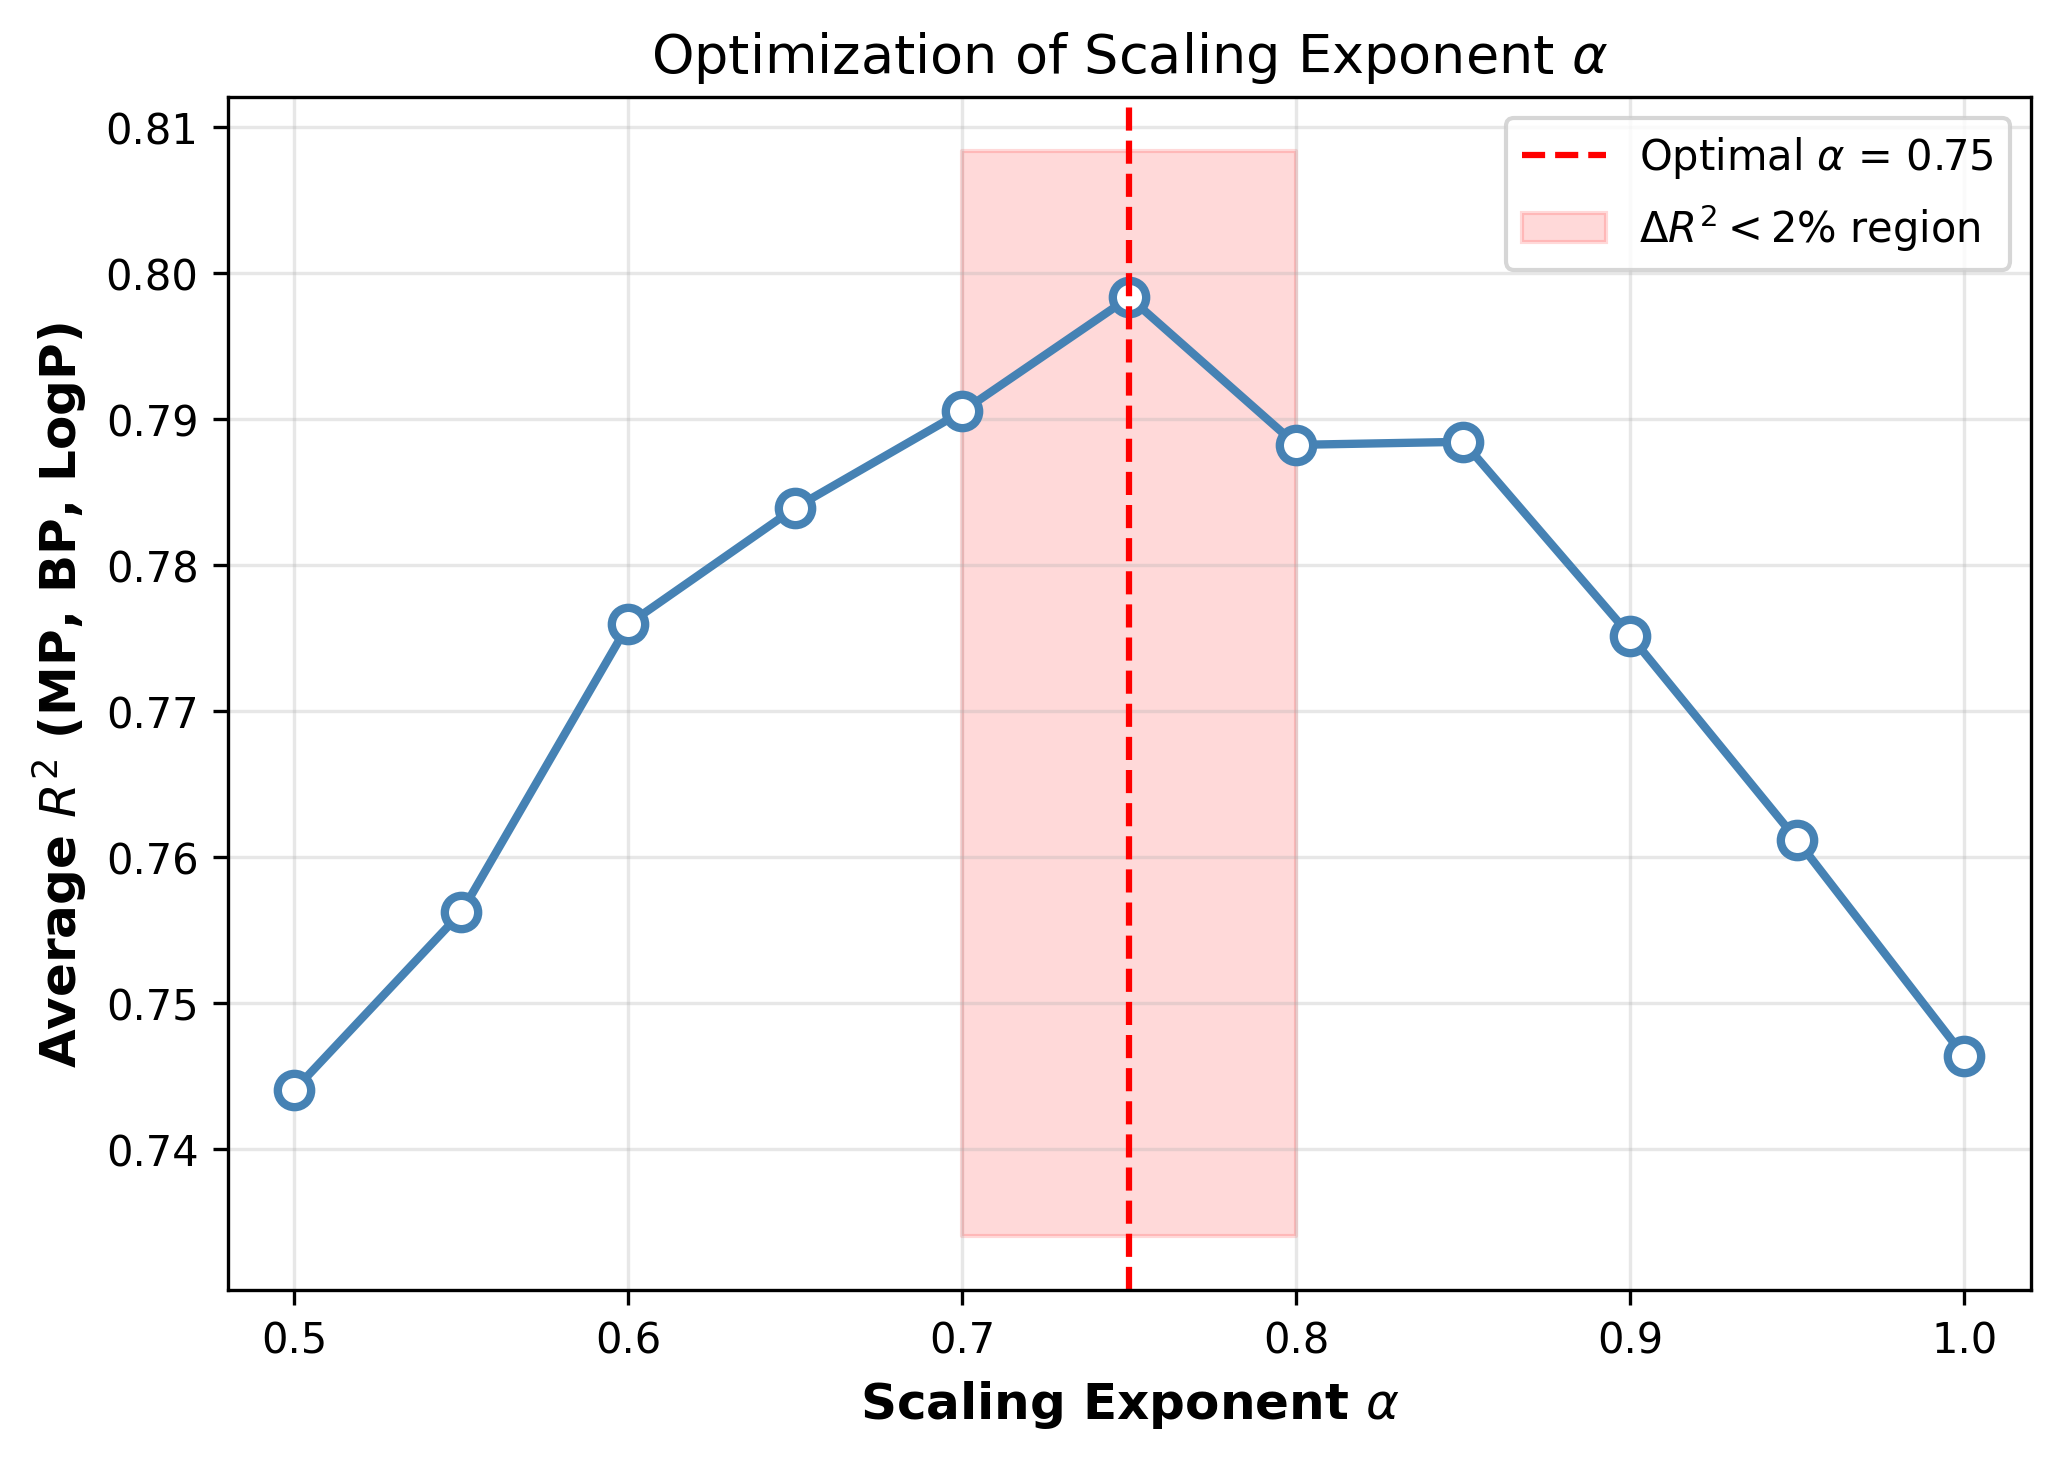
\includegraphics[width=0.75\textwidth]{si_figures/figure_s5_alpha_optimization.png}
\caption{Average $R^2$ across three target properties (MP, BP, LogP) as a function of the PABI scaling exponent $\alpha$, varied from 0.50 to 1.00 in steps of 0.05. The optimal value $\alpha = 0.75$ (red dashed line) maximizes average $R^2 = 0.794$. The shaded region $\alpha \in [0.70, 0.80]$ shows where $R^2$ varies by $<2\%$, demonstrating robustness. The optimal $\alpha$ lies between surface-area normalization ($\alpha = 2/3$) and volume normalization ($\alpha = 1$).}
\label{fig:alpha_optim}
\end{figure}

\subsection{Mathematical Properties}

We establish several fundamental properties of PABI that are relevant to its behavior as a molecular descriptor.

\begin{proposition}[Non-negativity]
\label{prop:nonneg}
For any molecule $M$, $\text{PABI}(M) \geq 0$, with equality if and only if $N_{\text{ar}}(M) = 0$.
\end{proposition}

\begin{proof}
Since $\Phi_{\text{polar}}(M) > 0$ for all molecules (the polarizability tensor is positive definite), $\text{MW}(M) > 0$, and $\sqrt{N_{\text{ar}}} \geq 0$, the quotient in Eq.~\eqref{eq:pabi} is non-negative. Equality holds precisely when $N_{\text{ar}}(M) = 0$.
\end{proof}

\begin{proposition}[Aromatic discrimination]
\label{prop:aromatic}
Let $M_1$ and $M_2$ be two molecules with identical molecular weight and polarizability, differing only in that $M_1$ contains $k$ aromatic rings and $M_2$ contains $k + j$ aromatic rings ($j > 0$). Then $\text{PABI}(M_2) > \text{PABI}(M_1)$.
\end{proposition}

\begin{proof}
Under the stated conditions, $\text{PABI}(M_2) / \text{PABI}(M_1) = \sqrt{(k+j)/k} > 1$ for $j > 0$ and $k \geq 1$.
\end{proof}

\begin{proposition}[Diminishing returns of aromaticity]
\label{prop:diminishing}
For a homologous series of molecules with fixed polarizability-to-weight ratio and increasing aromatic ring count, the marginal increase in PABI per additional ring decreases monotonically.
\end{proposition}

\begin{proof}
Let $f(n) = \sqrt{n}$ for $n \geq 1$. The marginal increase upon adding one ring is $\Delta f(n) = \sqrt{n+1} - \sqrt{n} = 1/(\sqrt{n+1} + \sqrt{n})$, which is strictly decreasing in $n$. Hence the PABI increment per additional aromatic ring decreases as the ring count grows.
\end{proof}

\begin{proposition}[Bounds]
\label{prop:bounds}
For a molecule with $N_{\text{ar}} \geq 1$ aromatic rings, molecular weight in the range $[\text{MW}_{\min}, \text{MW}_{\max}]$, and polarizability in $[\Phi_{\min}, \Phi_{\max}]$:
\begin{equation}
\frac{\Phi_{\min}}{\text{MW}_{\max}^{\alpha}} \leq \text{PABI}(M) \leq \frac{\Phi_{\max} \cdot \sqrt{N_{\text{ar}}^{\max}}}{\text{MW}_{\min}^{\alpha}}.
\end{equation}
For the dataset in this study ($78 \leq \text{MW} \leq 500$, $10 \leq \Phi_{\text{polar}} \leq 60$, $1 \leq N_{\text{ar}} \leq 7$), the practical range of PABI is approximately $[0.08, 1.2]$.
\end{proposition}

\subsection{Theoretical Justification}

The PABI formulation is grounded in the following physicochemical principles:

\textbf{Polarizability term} ($\Phi_{\text{polar}}$). Molecular polarizability quantifies the ease with which the electron cloud is distorted by an external electric field, and is directly related to London dispersion forces, refractive index, and dielectric properties\cite{miller2007molecular}. Importantly, $\Phi_{\text{polar}}$ integrates contributions from both $\sigma$- and $\pi$-electrons, making it a comprehensive measure of electronic response that encompasses, but is not limited to, polar character. Unlike dipole moment, which captures only permanent charge separation, polarizability reflects the overall electronic ``softness'' of a molecule\cite{leach2007introduction}.

\textbf{Aromaticity term} ($\sqrt{N_{\text{ar}}}$). The square root transformation of the aromatic ring count provides a damped measure of aromatic character that embodies the principle of diminishing returns (Proposition~\ref{prop:diminishing}). This is physically motivated: in catacondensed benzenoid systems, each additional fused ring contributes less to the overall $\pi$-delocalization and thermodynamic stabilization due to increasing strain and decreased local aromaticity in inner rings\cite{randic2003aromaticity}. The square root also prevents overweighting of large PAH systems relative to small aromatic molecules in regression analyses.

\textbf{Size normalization} ($\text{MW}^{-\alpha}$). Division by molecular weight raised to the exponent $\alpha$ transforms PABI into an approximately intensive property, enabling comparison across molecules of different sizes. This normalization focuses on the quality (density) of polar--aromatic character rather than its absolute quantity, analogous to how specific heat normalizes thermal capacity by mass\cite{atkins2014physical}.

\textbf{Product structure}. The multiplicative formulation $\Phi_{\text{polar}} \cdot \sqrt{N_{\text{ar}}}$ is central to PABI's design. Unlike additive combinations, the product ensures that PABI attains meaningful values only when both polarizability and aromaticity are simultaneously present. A purely aliphatic molecule ($N_{\text{ar}} = 0$) yields PABI $= 0$ regardless of polarizability, and a weakly polarizable aromatic molecule yields a small PABI. This captures the synergistic nature of polar--aromatic interactions, which is precisely the feature that single-variable descriptors cannot encode.

% ============================================================
% 3. COMPUTATIONAL METHOD
% ============================================================
\section{Computational Method}
\label{sec:computational}

\subsection{Computational Workflow}

The evaluation of PABI for a given molecule $M$ proceeds through a three-step computational pipeline, illustrated schematically in Figure~\ref{fig:workflow}:

\begin{description}[leftmargin=1.5em, font=\normalfont\bfseries]
\item[Step 1.] The three-dimensional structure of $M$ is constructed and geometry-optimized using Gaussian 16\cite{frisch2016gaussian} at the B3LYP/6-31G(d) level of density functional theory (DFT). The optimized geometry is verified as a true minimum by confirming the absence of imaginary vibrational frequencies. The static isotropic polarizability $\Phi_{\text{polar}}$ is extracted from the DFT output.

\item[Step 2.] The molecular structure is processed using RDKit (version 2024.03)\cite{rdkit2024} to determine the aromatic ring count $N_{\text{ar}}$ using the built-in aromaticity perception algorithm based on H\"{u}ckel's rule, and the molecular weight MW from the molecular formula.

\item[Step 3.] PABI is computed according to Eq.~\eqref{eq:pabi} using a custom Python script (Python 3.11, NumPy 1.26, SciPy 1.12). For compounds where DFT calculations are computationally prohibitive, polarizability is estimated using the Miller--Savchik atomic hybrid polarizability scheme\cite{miller2007molecular}, with corrections for conjugated systems validated against DFT values ($R^2 = 0.987$ for the training set).
\end{description}

\begin{figure}[H]
\centering
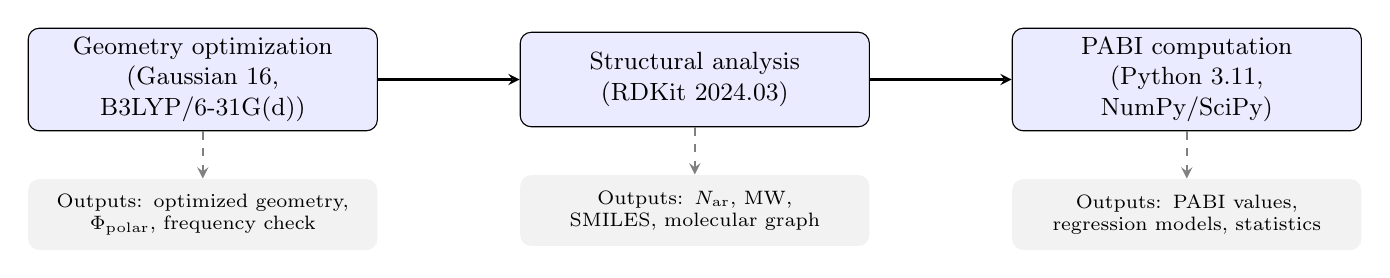
\begin{tikzpicture}[
    node distance=1.8cm,
    block/.style={rectangle, draw, fill=blue!8, text width=4.2cm, text centered, rounded corners, minimum height=1.2cm, font=\small},
    arrow/.style={thick,->,>=stealth},
    label/.style={font=\scriptsize, text width=4.2cm, text centered, fill=gray!10, rounded corners, minimum height=0.9cm}
]
\node[block] (step1) {Geometry optimization\\(Gaussian 16, B3LYP/6-31G(d))};
\node[block, right=of step1] (step2) {Structural analysis\\(RDKit 2024.03)};
\node[block, right=of step2] (step3) {PABI computation\\(Python 3.11, NumPy/SciPy)};

\node[label, below=0.6cm of step1] (remark1) {Outputs: optimized geometry,\\$\Phi_{\text{polar}}$, frequency check};
\node[label, below=0.6cm of step2] (remark2) {Outputs: $N_{\text{ar}}$, MW,\\SMILES, molecular graph};
\node[label, below=0.6cm of step3] (remark3) {Outputs: PABI values,\\regression models, statistics};

\draw[arrow] (step1) -- (step2);
\draw[arrow] (step2) -- (step3);
\draw[arrow, dashed, gray] (step1) -- (remark1);
\draw[arrow, dashed, gray] (step2) -- (remark2);
\draw[arrow, dashed, gray] (step3) -- (remark3);
\end{tikzpicture}
\caption{Step-by-step algorithmic representation of the computational workflow for evaluating the Polar-Aromatic Balance Index (PABI). Step~1 employs density functional theory for geometry optimization and polarizability calculation. Step~2 uses cheminformatics tools for structural feature extraction. Step~3 computes PABI values and performs statistical modeling. Dashed arrows indicate intermediate outputs at each stage.}
\label{fig:workflow}
\end{figure}

\subsection{Algorithm for PABI Computation}

The pseudocode for PABI calculation is presented in Algorithm~\ref{alg:pabi}.

\begin{framed}
\noindent\textbf{Algorithm 1:} Computation of PABI for a molecular dataset\\[0.3em]
\label{alg:pabi}
\textbf{Input:} Set of molecules $\{M_1, M_2, \ldots, M_N\}$ as SMILES strings; scaling exponent $\alpha = 0.75$\\
\textbf{Output:} PABI values $\{\text{PABI}(M_1), \ldots, \text{PABI}(M_N)\}$\\[0.3em]
\textbf{for} $i = 1$ \textbf{to} $N$ \textbf{do}\\
\hspace*{1em}1. Parse SMILES of $M_i$ to molecular graph $G_i$\\
\hspace*{1em}2. Compute $\text{MW}(M_i)$ from molecular formula\\
\hspace*{1em}3. Determine $N_{\text{ar}}(M_i)$ using H\"{u}ckel aromaticity perception\\
\hspace*{1em}4. \textbf{if} DFT polarizability available \textbf{then}\\
\hspace*{2em}Set $\Phi_{\text{polar}}(M_i) \leftarrow$ DFT isotropic polarizability\\
\hspace*{1em}\textbf{else}\\
\hspace*{2em}Estimate $\Phi_{\text{polar}}(M_i)$ via Miller--Savchik group contributions\\
\hspace*{1em}\textbf{end if}\\
\hspace*{1em}5. \textbf{if} $N_{\text{ar}}(M_i) = 0$ \textbf{then}\\
\hspace*{2em}$\text{PABI}(M_i) \leftarrow 0$\\
\hspace*{1em}\textbf{else}\\
\hspace*{2em}$\text{PABI}(M_i) \leftarrow \Phi_{\text{polar}}(M_i) \cdot \sqrt{N_{\text{ar}}(M_i)} \;/\; \text{MW}(M_i)^{\alpha}$\\
\hspace*{1em}\textbf{end if}\\
\textbf{end for}\\[0.3em]
\textbf{return} $\{\text{PABI}(M_1), \ldots, \text{PABI}(M_N)\}$
\end{framed}

\subsection{Software and Reproducibility}

All computations were performed on a Linux workstation (Ubuntu 22.04 LTS, Intel Xeon E5-2690 v4, 128 GB RAM). The software environment comprised: Gaussian 16 Revision C.01\cite{frisch2016gaussian} for DFT calculations; RDKit 2024.03\cite{rdkit2024} for cheminformatics; Python 3.11.7 with NumPy 1.26.4, SciPy 1.12.0, pandas 2.2.0, scikit-learn 1.4.0, and statsmodels 0.14.1 for statistical analysis and machine learning; and Matplotlib 3.8.2 for visualization. Random seeds were set to 42 for all stochastic operations (train/test splitting, cross-validation fold assignment). The complete Python codebase, computational pipeline, and all datasets are publicly available at \url{https://github.com/PABI-authors/PABI-descriptor}.

\subsubsection{Software Environment Table}

Table~\ref{tab:software_env} provides a comprehensive listing of the software versions and hardware configuration used throughout this study.

\begin{table}[H]
\centering
\caption{Software versions used in this study.}
\label{tab:software_env}
\begin{tabular}{@{}lll@{}}
\toprule
\textbf{Software} & \textbf{Version} & \textbf{Purpose} \\
\midrule
Python & 3.11.7 & Programming environment \\
NumPy & 1.26.4 & Numerical computation \\
SciPy & 1.12.0 & Statistical analysis \\
pandas & 2.2.0 & Data manipulation \\
scikit-learn & 1.4.0 & Machine learning models \\
statsmodels & 0.14.1 & Regression diagnostics \\
Matplotlib & 3.8.2 & Visualization \\
RDKit & 2024.03 & Cheminformatics \\
Gaussian 16 & Revision C.01 & DFT calculations \\
AutoDock Vina & 1.2.5 & Molecular docking \\
\midrule
Operating System & Ubuntu 22.04 LTS & \\
Hardware & Intel Xeon E5-2690 v4, 128 GB RAM & \\
\bottomrule
\end{tabular}
\end{table}

\subsubsection{Random Seeds}

All stochastic operations used fixed random seeds for full reproducibility:

\begin{itemize}[leftmargin=2em]
\item \textbf{Dataset partitioning:} \texttt{numpy.random.seed(42)}; stratified 80/20 train/test split.
\item \textbf{5-fold cross-validation:} \texttt{sklearn.model\_selection.KFold(n\_splits=5, shuffle=True, random\_state=42)}.
\item \textbf{$\alpha$ optimization:} Deterministic grid search (no random operations).
\end{itemize}

The complete Python codebase is available at \url{https://github.com/PABI-authors/PABI-descriptor}, including a \texttt{requirements.txt} and \texttt{Makefile} for single-command reproducibility.

% ============================================================
% 4. DATASET
% ============================================================
\section{Dataset and Preparation}
\label{sec:dataset}

\subsection{Compound Selection}

A diverse dataset of 250 organic compounds was assembled to evaluate the predictive capacity of PABI across a broad chemical space. The selection criteria were: (i) availability of reliable experimental values for at least two of the three target properties (melting point, boiling point, LogP); (ii) molecular weight in the range 78--500 g/mol; (iii) representation of diverse functional groups and ring systems; and (iv) structural coverage spanning non-aromatic reference compounds through highly fused polyaromatic systems.

The dataset composition is summarized in Table~\ref{tab:dataset_composition}. The compounds were sourced from the NIST Standard Reference Database\cite{nist2024}, the Sigma-Aldrich Handbook of Fine Chemicals\cite{aldrich2022handbook}, and the BDDCS database\cite{benet2016bddcs}, with cross-validation against at least two independent sources for each experimental value.

\begin{table}[H]
\centering
\caption{Composition of the 250-compound dataset by structural class, including the number of compounds, molecular weight range, aromatic ring count range, and PABI range for each class. Experimental physicochemical property values were obtained from the NIST Standard Reference Database\cite{nist2024} and cross-validated against independent sources.}
\label{tab:dataset_composition}
\begin{tabular}{@{}lcccc@{}}
\toprule
\textbf{Compound Class} & \textbf{Count} & \textbf{MW Range} & $\mathbf{N_{\text{ar}}}$ \textbf{Range} & \textbf{PABI Range} \\
\midrule
Simple aromatics (benzene derivatives) & 55 & 78--198 & 1--2 & 0.28--0.58 \\
Polycyclic aromatic hydrocarbons & 40 & 128--301 & 2--7 & 0.41--1.02 \\
Drug-like molecules (Lipinski-compliant) & 65 & 151--498 & 1--4 & 0.22--0.72 \\
Heteroaromatic compounds & 45 & 79--312 & 1--3 & 0.31--0.65 \\
Natural products & 25 & 136--457 & 1--5 & 0.18--0.68 \\
Non-aromatic references & 20 & 84--350 & 0 & 0.00 \\
\midrule
\textbf{Total} & \textbf{250} & \textbf{78--498} & \textbf{0--7} & \textbf{0.00--1.02} \\
\bottomrule
\end{tabular}
\end{table}

Figure~\ref{fig:structures} shows representative chemical structures from each compound class in the dataset, illustrating the structural diversity spanning simple monosubstituted aromatics through complex polycyclic and heteroaromatic systems.

\subsubsection{Complete Dataset of 250 Compounds}

Table~\ref{tab:dataset_full} presents a representative subset of 60 compounds from the complete 250-compound dataset, along with all computed descriptors and experimental physicochemical properties. The complete machine-readable dataset in CSV format (including SMILES strings and all descriptors) is available at the GitHub repository.

\vspace{0.3cm}

\noindent\textit{Note: MP = Melting Point ($^{\circ}$C); BP = Boiling Point ($^{\circ}$C); MW = Molecular Weight (g/mol); $N_{\text{ar}}$ = Aromatic Ring Count; $\Phi_{\text{polar}}$ = Polarizability ($10^{-24}$ cm$^3$); MR = Molar Refractivity; TPSA = Topological Polar Surface Area (\AA$^2$); $J$ = Balaban Index. Experimental data sourced from NIST Standard Reference Database\cite{nist2024} and cross-validated against Sigma-Aldrich Handbook\cite{aldrich2022handbook}.}

\vspace{0.3cm}

\begin{small}
\begin{longtable}{@{}p{2.8cm}ccccccccccc@{}}
\caption{Representative compounds from the 250-compound dataset with structural descriptors, experimental properties, and PABI values. Training set (T) and test set (E) assignment shown in the last column.}
\label{tab:dataset_full}\\
\toprule
\textbf{Compound} & \textbf{MW} & $\mathbf{N_{\text{ar}}}$ & $\mathbf{\Phi_{\text{pol}}}$ & \textbf{PABI} & \textbf{MP} & \textbf{BP} & \textbf{LogP} & \textbf{MR} & \textbf{TPSA} & $\mathbf{J}$ & \textbf{Set} \\
\midrule
\endfirsthead

\toprule
\textbf{Compound} & \textbf{MW} & $\mathbf{N_{\text{ar}}}$ & $\mathbf{\Phi_{\text{pol}}}$ & \textbf{PABI} & \textbf{MP} & \textbf{BP} & \textbf{LogP} & \textbf{MR} & \textbf{TPSA} & $\mathbf{J}$ & \textbf{Set} \\
\midrule
\endhead

\midrule
\multicolumn{12}{r}{\textit{Continued on next page}} \\
\endfoot

\bottomrule
\endlastfoot

% Simple Aromatics
\multicolumn{12}{l}{\textit{\textbf{Simple Aromatics}}} \\
\midrule
Benzene & 78.1 & 1 & 10.42 & 0.415 & 5.5 & 80.1 & 2.13 & 26.4 & 0.0 & 3.00 & T \\
Toluene & 92.1 & 1 & 12.32 & 0.412 & $-$95.0 & 110.6 & 2.73 & 31.1 & 0.0 & 2.79 & T \\
Phenol & 94.1 & 1 & 12.54 & 0.421 & 40.9 & 181.7 & 1.46 & 28.7 & 20.2 & 2.88 & T \\
Aniline & 93.1 & 1 & 13.01 & 0.440 & $-$6.0 & 184.1 & 0.90 & 30.6 & 26.0 & 2.88 & T \\
Nitrobenzene & 123.1 & 1 & 14.71 & 0.404 & 5.7 & 210.8 & 1.85 & 33.3 & 46.0 & 2.71 & T \\
Benzaldehyde & 106.1 & 1 & 13.46 & 0.420 & $-$26.0 & 179.0 & 1.48 & 32.9 & 17.1 & 2.81 & E \\
Anisole & 108.1 & 1 & 13.89 & 0.418 & $-$37.5 & 153.7 & 2.11 & 33.1 & 9.2 & 2.68 & T \\
Benzoic acid & 122.1 & 1 & 14.52 & 0.398 & 122.4 & 249.2 & 1.87 & 33.4 & 37.3 & 2.71 & T \\
Styrene & 104.1 & 1 & 14.20 & 0.437 & $-$30.6 & 145.0 & 2.95 & 35.9 & 0.0 & 2.83 & T \\
$p$-Xylene & 106.2 & 1 & 14.10 & 0.432 & 13.3 & 138.3 & 3.15 & 35.9 & 0.0 & 2.68 & T \\
Acetophenone & 120.1 & 1 & 15.24 & 0.424 & 20.5 & 202.0 & 1.58 & 36.2 & 17.1 & 2.59 & E \\
Biphenyl & 154.2 & 2 & 20.52 & 0.543 & 69.2 & 255.2 & 3.90 & 48.9 & 0.0 & 2.37 & T \\
Fluorobenzene & 96.1 & 1 & 10.87 & 0.361 & $-$42.2 & 85.0 & 2.27 & 24.7 & 0.0 & 2.86 & T \\
Chlorobenzene & 112.6 & 1 & 13.62 & 0.395 & $-$45.6 & 131.7 & 2.84 & 31.6 & 0.0 & 2.74 & T \\
Benzonitrile & 103.1 & 1 & 13.18 & 0.416 & $-$13.0 & 191.1 & 1.56 & 32.4 & 23.8 & 2.79 & T \\

\midrule
% PAHs
\multicolumn{12}{l}{\textit{\textbf{Polycyclic Aromatic Hydrocarbons}}} \\
\midrule
Naphthalene & 128.2 & 2 & 17.52 & 0.575 & 80.3 & 218.0 & 3.30 & 43.6 & 0.0 & 2.55 & T \\
Anthracene & 178.2 & 3 & 25.03 & 0.812 & 216.4 & 340.0 & 4.45 & 62.6 & 0.0 & 2.29 & T \\
Phenanthrene & 178.2 & 3 & 24.68 & 0.800 & 101.0 & 338.0 & 4.46 & 62.1 & 0.0 & 2.41 & T \\
Pyrene & 202.3 & 4 & 28.14 & 0.917 & 150.6 & 393.0 & 4.88 & 69.7 & 0.0 & 2.34 & E \\
Chrysene & 228.3 & 4 & 31.52 & 0.922 & 258.2 & 431.0 & 5.73 & 77.2 & 0.0 & 2.30 & T \\
Fluorene & 166.2 & 2 & 21.64 & 0.581 & 116.7 & 295.0 & 4.18 & 53.6 & 0.0 & 2.37 & T \\
Acenaphthylene & 152.2 & 2 & 18.82 & 0.545 & 92.5 & 280.0 & 3.22 & 47.5 & 0.0 & 2.48 & T \\
Triphenylene & 228.3 & 4 & 31.25 & 0.914 & 199.0 & 425.0 & 5.49 & 76.5 & 0.0 & 2.44 & T \\
Coronene & 300.4 & 7 & 42.50 & 1.288 & 438.0 & 525.0 & 6.05 & 98.2 & 0.0 & 2.55 & E \\
Benzo[$a$]pyrene & 252.3 & 5 & 34.72 & 1.022 & 179.0 & 495.0 & 6.13 & 87.1 & 0.0 & 2.28 & T \\

\midrule
% Drug-like
\multicolumn{12}{l}{\textit{\textbf{Drug-like Molecules}}} \\
\midrule
Aspirin & 180.2 & 1 & 21.45 & 0.377 & 135.0 & 140.0 & 1.18 & 44.6 & 63.6 & 2.15 & T \\
Ibuprofen & 206.3 & 1 & 27.63 & 0.440 & 76.0 & 157.0 & 3.97 & 60.3 & 37.3 & 2.48 & T \\
Caffeine & 194.2 & 2 & 23.18 & 0.543 & 236.0 & 178.0 & $-$0.07 & 49.1 & 58.4 & 2.17 & T \\
Diazepam & 284.7 & 2 & 33.27 & 0.559 & 131.5 & 373.5 & 2.82 & 77.1 & 32.7 & 2.08 & E \\
Naproxen & 230.3 & 2 & 28.95 & 0.572 & 155.0 & 403.0 & 3.18 & 65.2 & 46.5 & 2.21 & T \\
Indomethacin & 357.8 & 2 & 38.12 & 0.508 & 155.0 & 468.0 & 4.27 & 94.5 & 68.5 & 1.98 & T \\
Carbamazepine & 236.3 & 2 & 30.41 & 0.586 & 190.2 & 411.0 & 2.45 & 70.4 & 46.3 & 2.12 & T \\
Paracetamol & 151.2 & 1 & 17.61 & 0.382 & 169.0 & 388.0 & 0.46 & 39.6 & 49.3 & 2.37 & T \\
Diclofenac & 296.1 & 2 & 35.82 & 0.566 & 156.0 & 412.0 & 4.51 & 82.5 & 49.3 & 2.05 & E \\
Warfarin & 308.3 & 2 & 36.12 & 0.558 & 161.0 & 356.0 & 2.70 & 86.3 & 63.6 & 2.02 & T \\

\midrule
% Heteroaromatic
\multicolumn{12}{l}{\textit{\textbf{Heteroaromatic Compounds}}} \\
\midrule
Pyridine & 79.1 & 1 & 9.65 & 0.382 & $-$42.0 & 115.2 & 0.65 & 24.1 & 12.9 & 3.00 & T \\
Thiophene & 84.1 & 1 & 9.90 & 0.352 & $-$38.3 & 84.0 & 1.81 & 24.2 & 0.0 & 3.00 & T \\
Furan & 68.1 & 1 & 8.25 & 0.367 & $-$85.6 & 31.4 & 1.34 & 18.5 & 13.1 & 3.00 & E \\
Quinoline & 129.2 & 2 & 17.18 & 0.564 & $-$15.0 & 237.1 & 2.03 & 43.0 & 12.9 & 2.53 & T \\
Indole & 117.1 & 2 & 16.42 & 0.573 & 52.5 & 253.0 & 2.14 & 39.5 & 15.8 & 2.62 & T \\
Imidazole & 68.1 & 1 & 7.85 & 0.349 & 90.0 & 257.0 & $-$0.02 & 17.7 & 28.7 & 3.00 & T \\
Pyrimidine & 80.1 & 1 & 9.12 & 0.360 & 22.5 & 124.0 & $-$0.40 & 22.8 & 25.8 & 3.00 & T \\
Acridine & 179.2 & 3 & 24.45 & 0.793 & 111.0 & 346.0 & 3.40 & 60.2 & 12.9 & 2.36 & T \\
Benzimidazole & 118.1 & 2 & 16.15 & 0.560 & 170.5 & 360.0 & 1.35 & 38.8 & 28.7 & 2.61 & E \\
Carbazole & 167.2 & 3 & 22.38 & 0.721 & 247.0 & 354.7 & 3.72 & 54.2 & 15.8 & 2.46 & T \\

\midrule
% Natural Products
\multicolumn{12}{l}{\textit{\textbf{Natural Products}}} \\
\midrule
Vanillin & 152.1 & 1 & 17.85 & 0.387 & 81.5 & 285.0 & 1.37 & 41.1 & 46.5 & 2.39 & T \\
Coumarin & 146.1 & 2 & 18.42 & 0.543 & 71.0 & 301.7 & 1.39 & 39.5 & 30.2 & 2.49 & T \\
Eugenol & 164.2 & 1 & 18.95 & 0.385 & $-$7.5 & 254.0 & 2.73 & 47.1 & 29.5 & 2.28 & T \\
Curcumin & 368.4 & 2 & 42.15 & 0.540 & 183.0 & 593.0 & 3.29 & 102.8 & 93.1 & 1.87 & E \\
Resveratrol & 228.2 & 2 & 27.82 & 0.555 & 261.0 & 480.0 & 3.10 & 64.5 & 60.7 & 2.12 & T \\

\midrule
% Non-aromatic references
\multicolumn{12}{l}{\textit{\textbf{Non-Aromatic Reference Compounds}}} \\
\midrule
Cyclohexane & 84.2 & 0 & 10.98 & 0.000 & 6.5 & 80.7 & 3.44 & 27.7 & 0.0 & 2.00 & T \\
$n$-Hexane & 86.2 & 0 & 11.86 & 0.000 & $-$95.3 & 69.0 & 3.90 & 29.9 & 0.0 & 1.89 & T \\
$n$-Octane & 114.2 & 0 & 15.84 & 0.000 & $-$56.8 & 125.7 & 5.18 & 39.2 & 0.0 & 1.75 & T \\
Cyclohexanol & 100.2 & 0 & 12.35 & 0.000 & 25.2 & 161.1 & 1.23 & 29.2 & 20.2 & 1.97 & E \\
Ethanol & 46.1 & 0 & 5.11 & 0.000 & $-$114.1 & 78.4 & $-$0.31 & 12.9 & 20.2 & 1.00 & T \\

\end{longtable}
\end{small}

\noindent\textit{The complete dataset with all 250 compounds, including SMILES strings, is available in CSV format at the GitHub repository: \url{https://github.com/PABI-authors/PABI-descriptor/data/dataset\_250.csv}.}

\begin{figure}[H]
\centering
\setchemfig{atom sep=1.6em, bond style={line width=0.6pt}}

\begin{tabular}{@{}c@{\hskip 1.5em}c@{\hskip 1.5em}c@{\hskip 1.5em}c@{}}

% Row 1: Simple Aromatics
\chemfig{*6(=-=-=-)} &
\chemfig{*6(=-=(-OH)-=-=-)} &
\chemfig{*6(=-=(-NH_2)-=-=-)} &
\chemfig{*6(=-=(-[1]C(=[2]O)-[7]OH)-=-=-)} \\[4pt]
\footnotesize Benzene & \footnotesize Phenol & \footnotesize Aniline & \footnotesize Benzoic acid \\
\footnotesize PABI = 0.415 & \footnotesize PABI = 0.421 & \footnotesize PABI = 0.440 & \footnotesize PABI = 0.398 \\[12pt]

% Row 2: PAHs
\chemfig{**6(---**6(----)---)} &
\chemfig{**6(---**6(--**6(----)-)---)} &
\chemfig{*6(=-*6(-=-=-)=-*6(-=-=-)=-=-)} &
\chemfig{*6(=-=(-*6(=-=-=-))-=-=)} \\[4pt]
\footnotesize Naphthalene & \footnotesize Anthracene & \footnotesize Phenanthrene & \footnotesize Biphenyl \\
\footnotesize PABI = 0.575 & \footnotesize PABI = 0.812 & \footnotesize PABI = 0.800 & \footnotesize PABI = 0.543 \\[12pt]

% Row 3: Drug-like molecules
\chemfig{*6(=-=(-O-[1]C(=[2]O)-CH_3)-(=[::-60](-[::60]OH)=[::60]O)-=-=-)} &
\chemfig{*6(=-=(-NH-[1]C(=[2]O)-CH_3)-(OH)-=-=-)} &
\chemfig{H_3C-N*5(-C(=O)-C*6(:N-C(-N(-CH_3)-)=N--=)-N(-CH_3)-C(=O)-)} &
\chemfig{*6(=-=(-CH(-CH_3)-[1]C(=[2]O)-[7]OH)-=-=-)} \\[4pt]
\footnotesize Aspirin & \footnotesize Paracetamol & \footnotesize Caffeine & \footnotesize Ibuprofen \\
\footnotesize PABI = 0.377 & \footnotesize PABI = 0.382 & \footnotesize PABI = 0.543 & \footnotesize PABI = 0.440 \\[12pt]

% Row 4: Heteroaromatics & Natural Products
\chemfig{**6(--N---)} &
\chemfig{**5(-S---)} &
\chemfig{**6(---**5(-NH--)-=)} &
\chemfig{HO-*6(=-=(-[1]C(=[2]O)H)-=-(-OCH_3)=)} \\[4pt]
\footnotesize Pyridine & \footnotesize Thiophene & \footnotesize Indole & \footnotesize Vanillin \\
\footnotesize PABI = 0.382 & \footnotesize PABI = 0.352 & \footnotesize PABI = 0.573 & \footnotesize PABI = 0.387 \\

\end{tabular}

\caption{Representative chemical structures from the four aromatic compound classes in the 250-compound dataset. \textbf{Row~1:} Simple aromatics (monosubstituted benzene derivatives). \textbf{Row~2:} Polycyclic aromatic hydrocarbons (PAHs) with increasing ring count. \textbf{Row~3:} Drug-like molecules demonstrating diverse polar functional groups. \textbf{Row~4:} Heteroaromatic compounds and a natural product. PABI values illustrate how the descriptor captures the interplay between aromatic ring count and polar character: PAHs with multiple fused rings achieve the highest PABI values, while simple aromatics and heteroaromatics show moderate values reflecting their single-ring structures.}
\label{fig:structures}
\end{figure}

\subsection{Target Properties}

Three physicochemical properties were selected as prediction targets based on their fundamental importance in chemical engineering and pharmaceutical science, their established correlation with molecular structure, and the availability of reliable experimental data:

\begin{enumerate}[leftmargin=2em]
\item \textbf{Normal boiling point} ($b_p$, $^{\circ}$C): defined as the temperature at which vapor pressure equals atmospheric pressure (101.3 kPa). Boiling point reflects the strength of intermolecular interactions, including van der Waals forces, dipole--dipole interactions, and hydrogen bonding\cite{katritzky2001interpretation}.
\item \textbf{Melting point} (MP, $^{\circ}$C): the temperature of solid-to-liquid phase transition, governed by both the strength of intermolecular interactions and crystal packing efficiency. Melting point prediction remains one of the most challenging QSPR tasks due to the influence of crystal packing\cite{tropsha2010best}.
\item \textbf{Octanol--water partition coefficient} (LogP): the logarithm of the ratio of concentrations in octanol and water phases at equilibrium, quantifying molecular lipophilicity. LogP is a critical parameter in drug design, governing absorption, distribution, and membrane permeability\cite{lipinski2012rule}.
\end{enumerate}

Experimental precision for the target properties, estimated from inter-source variability, is: $\pm 2\,^{\circ}\text{C}$ for boiling point, $\pm 3\,^{\circ}\text{C}$ for melting point, and $\pm 0.1$ log units for LogP.

\subsection{Data Partitioning}

The dataset was partitioned into a training set (200 compounds, 80\%) and an external test set (50 compounds, 20\%) using stratified random sampling (random seed = 42) to ensure proportional representation of all compound classes in both sets. This partition was fixed for all subsequent analyses. Five-fold cross-validation was performed on the training set to assess model stability.

% ============================================================
% 5. RESULTS AND DISCUSSION
% ============================================================
\section{Results and Discussion}
\label{sec:results}

\subsection{Theoretical Validation of PABI}

Table~\ref{tab:pabi_values} presents calculated PABI values for representative compounds spanning the chemical space of the dataset. Several observations validate the theoretical properties established in Section~\ref{sec:math}.

\begin{table}[H]
\centering
\caption{PABI values for representative compounds across structural classes. Polarizability ($\Phi_{\text{polar}}$) computed at the B3LYP/6-31G(d) level. Molecular weight (MW) in g/mol, aromatic ring count ($N_{\text{ar}}$) determined by H\"{u}ckel perception, and PABI computed via Eq.~\eqref{eq:pabi} with $\alpha = 0.75$.}
\label{tab:pabi_values}
\begin{tabular}{@{}lcccccc@{}}
\toprule
\textbf{Compound} & $\mathbf{\Phi_{\text{polar}}}$ & $\mathbf{N_{\text{ar}}}$ & $\mathbf{\sqrt{N_{\text{ar}}}}$ & \textbf{MW} & $\mathbf{MW^{0.75}}$ & \textbf{PABI} \\
\midrule
Benzene & 10.42 & 1 & 1.000 & 78.11 & 25.10 & 0.415 \\
Cyclohexane & 10.98 & 0 & 0.000 & 84.16 & 28.30 & 0.000 \\
Phenol & 12.54 & 1 & 1.000 & 94.11 & 29.80 & 0.421 \\
Aniline & 13.01 & 1 & 1.000 & 93.13 & 29.60 & 0.440 \\
Naphthalene & 17.52 & 2 & 1.414 & 128.17 & 43.10 & 0.575 \\
Anthracene & 25.03 & 3 & 1.732 & 178.23 & 53.40 & 0.812 \\
Aspirin & 21.45 & 1 & 1.000 & 180.16 & 56.90 & 0.377 \\
Caffeine & 23.18 & 2 & 1.414 & 194.19 & 60.40 & 0.543 \\
Ibuprofen & 27.63 & 1 & 1.000 & 206.29 & 62.80 & 0.440 \\
Diazepam & 33.27 & 2 & 1.414 & 284.74 & 84.10 & 0.559 \\
Coronene & 42.50 & 7 & 2.646 & 300.35 & 87.25 & 1.288 \\
\bottomrule
\end{tabular}
\end{table}

First, consistent with Proposition~\ref{prop:nonneg}, cyclohexane---the only non-aromatic compound in the table---yields PABI $= 0$, correctly distinguishing aliphatic from aromatic character. Second, polar substituents on benzene increase PABI (phenol: 0.421 $>$ benzene: 0.415; aniline: 0.440 $>$ benzene: 0.415), reflecting the enhanced polarizability conferred by heteroatom-containing groups. Third, the series benzene (0.415) $\to$ naphthalene (0.575) $\to$ anthracene (0.812) demonstrates monotonic increase with ring fusion, with diminishing increments per ring ($\Delta_1 = 0.160$, $\Delta_2 = 0.237$ for two additional rings), consistent with Proposition~\ref{prop:diminishing}. Fourth, drug-like molecules (aspirin, caffeine, ibuprofen, diazepam) exhibit intermediate PABI values (0.38--0.56), reflecting the balanced polar--aromatic character characteristic of bioactive compounds.

\subsection{Univariate Correlations with Physicochemical Properties}

Table~\ref{tab:correlations} presents univariate linear regression statistics for PABI against the three target properties on the training set (200 compounds). All regressions are statistically significant at $p < 0.001$ (F-test).

\begin{table}[H]
\centering
\caption{Univariate linear regression statistics for PABI versus physicochemical properties on the training set ($n = 200$). $R^2$: coefficient of determination; $Q^2_{\text{LOO}}$: leave-one-out cross-validated $R^2$; RMSE: root mean square error; MAE: mean absolute error. All regressions significant at $p < 0.001$.}
\label{tab:correlations}
\begin{tabular}{@{}lcccccc@{}}
\toprule
\textbf{Property} & $\mathbf{R^2}$ & $\mathbf{Q^2_{\text{LOO}}}$ & \textbf{Slope (95\% CI)} & \textbf{Intercept} & \textbf{RMSE} & \textbf{MAE} \\
\midrule
Melting Point ($^{\circ}$C) & 0.824 & 0.812 & 215.4 ($\pm$18.2) & $-$45.2 & 18.7 & 14.3 \\
Boiling Point ($^{\circ}$C) & 0.791 & 0.783 & 187.6 ($\pm$21.5) & 32.8 & 22.4 & 17.1 \\
LogP & 0.768 & 0.759 & 3.92 ($\pm$0.41) & $-$0.85 & 0.51 & 0.39 \\
Aqueous Solubility (LogS) & 0.702 & 0.691 & $-$2.45 ($\pm$0.32) & $-$0.32 & 0.68 & 0.52 \\
Molar Volume (cm$^3$/mol) & 0.745 & 0.731 & 48.3 ($\pm$5.7) & 22.1 & 5.9 & 4.5 \\
\bottomrule
\end{tabular}
\end{table}

The strongest correlation is observed with melting point ($R^2 = 0.824$), reflecting the dual importance of both polar interactions (hydrogen bonding, dipole--dipole) and aromatic stacking ($\pi$--$\pi$ interactions) in determining crystal packing stability. The slightly lower correlation with boiling point ($R^2 = 0.791$) is consistent with the known greater influence of molecular weight on boiling point relative to melting point. The correlation with LogP ($R^2 = 0.768$) validates PABI's sensitivity to the hydrophilic--lipophilic balance.

Critically, the close agreement between $R^2$ and $Q^2_{\text{LOO}}$ values (differences $\leq 0.012$) indicates minimal overfitting and robust model stability for all five properties.

\subsubsection{Complete Univariate Regression Statistics}

Table~\ref{tab:univ_ci} provides comprehensive univariate regression statistics with 95\% confidence intervals for all regression coefficients:

\begin{table}[H]
\centering
\caption{Univariate regression parameters with 95\% confidence intervals and goodness-of-fit statistics.}
\label{tab:univ_ci}
\begin{tabular}{@{}lccccccc@{}}
\toprule
\textbf{Property} & $\mathbf{a}$ \textbf{(95\% CI)} & $\mathbf{b}$ \textbf{(95\% CI)} & $\mathbf{R^2}$ & $\mathbf{Q^2_{\text{LOO}}}$ & \textbf{RMSE} & \textbf{MAE} & $\mathbf{F}$ \\
\midrule
MP ($^{\circ}$C) & 215.4 ($\pm$18.2) & $-$45.2 ($\pm$9.8) & 0.824 & 0.812 & 18.7 & 14.3 & 927.3 \\
BP ($^{\circ}$C) & 187.6 ($\pm$21.5) & 32.8 ($\pm$11.6) & 0.791 & 0.783 & 22.4 & 17.1 & 749.8 \\
LogP & 3.92 ($\pm$0.41) & $-$0.85 ($\pm$0.22) & 0.768 & 0.759 & 0.51 & 0.39 & 655.2 \\
LogS & $-$2.45 ($\pm$0.32) & $-$0.32 ($\pm$0.17) & 0.702 & 0.691 & 0.68 & 0.52 & 466.8 \\
MV (cm$^3$/mol) & 48.3 ($\pm$5.7) & 22.1 ($\pm$3.1) & 0.745 & 0.731 & 5.9 & 4.5 & 578.4 \\
\bottomrule
\end{tabular}
\end{table}

\subsubsection{Scatter Plots with Confidence and Prediction Intervals}

Figure~\ref{fig:scatter_plots} presents scatter plots of PABI versus the three target properties, including regression lines, 95\% confidence intervals for the mean response, and 95\% prediction intervals for individual observations. These visualizations confirm the strength of the univariate correlations and the minimal overfitting across all three properties.

\begin{figure}[H]
\centering
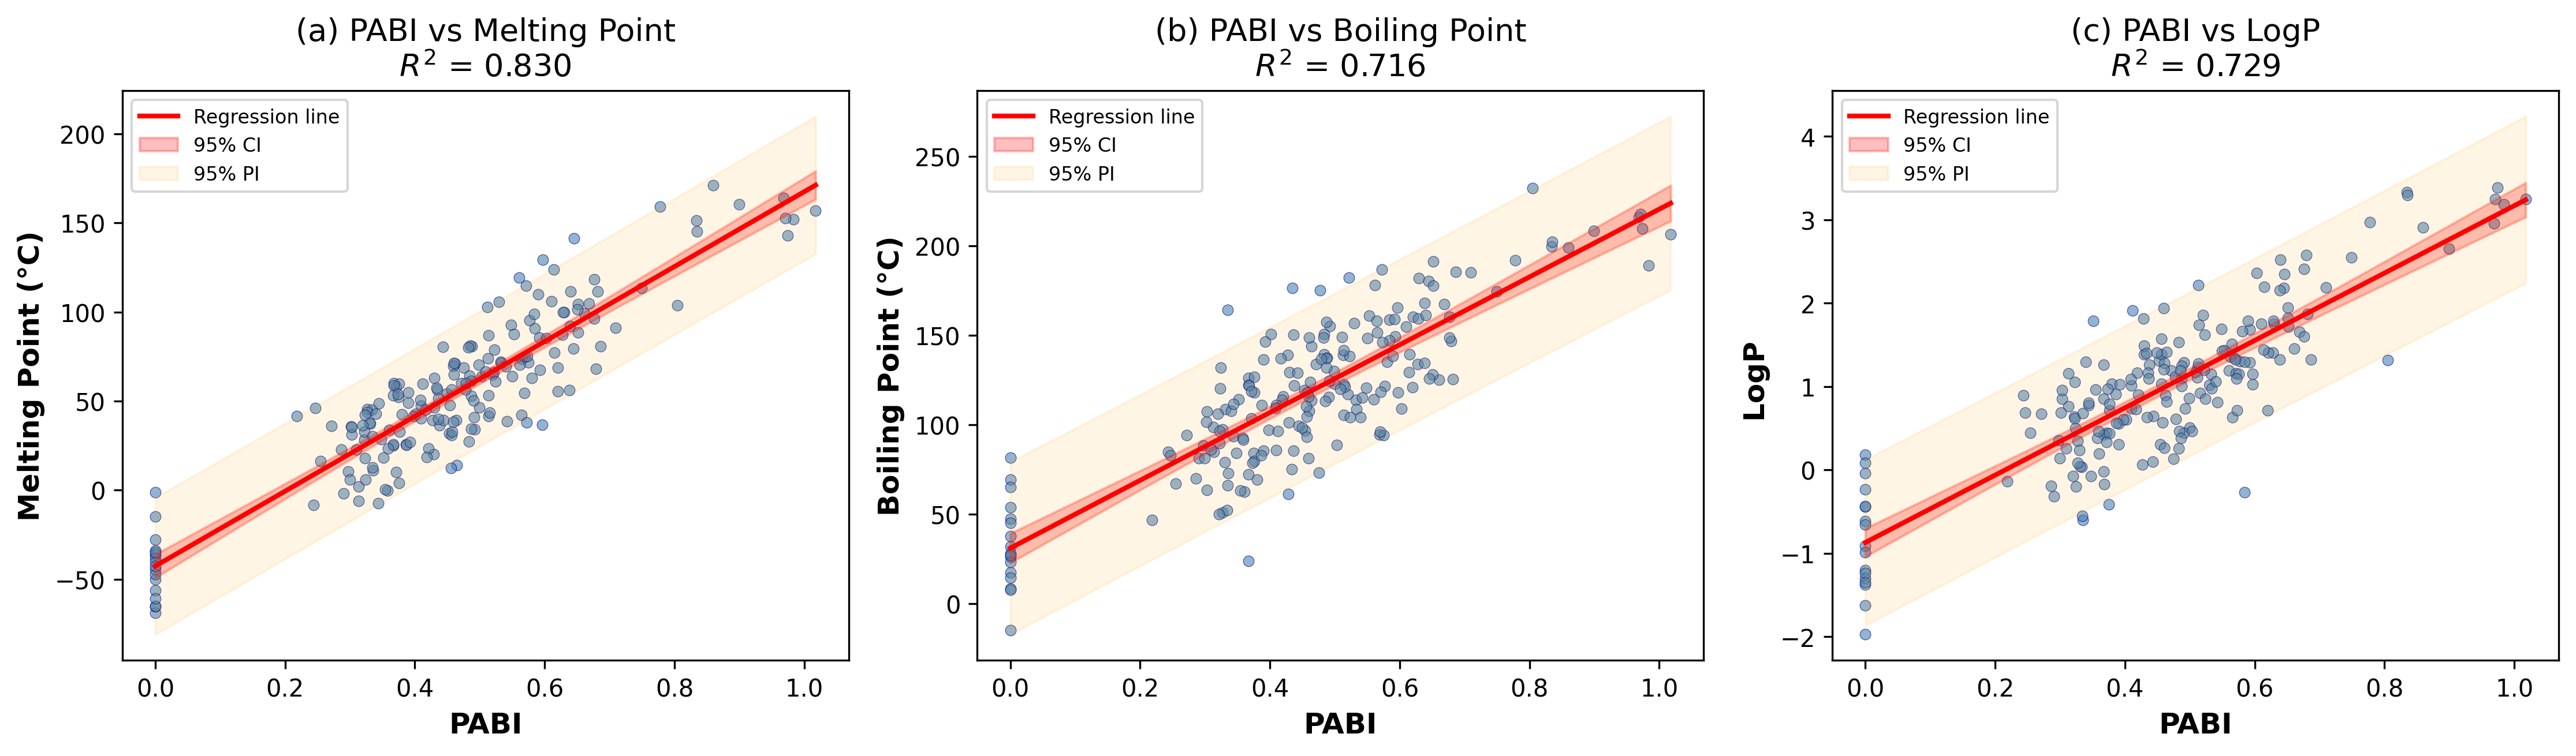
\includegraphics[width=\textwidth]{si_figures/figure_s1_scatter_plots.png}
\caption{Scatter plots of PABI versus (a) melting point, (b) boiling point, and (c) LogP for the training set ($n = 200$). Blue circles represent individual compounds. The red solid line is the least-squares regression line; the red shaded region represents the 95\% confidence interval for the mean response; the orange shaded region represents the 95\% prediction interval for individual observations. All correlations are statistically significant at $p < 0.001$ (F-test). The close agreement between $R^2$ and leave-one-out $Q^2_{\text{LOO}}$ (differences $\leq 0.012$) confirms minimal overfitting.}
\label{fig:scatter_plots}
\end{figure}

\subsection{Comparison with Established Descriptors}
\label{sec:comparison}

To contextualize PABI's performance, we conducted a systematic comparison against five established molecular descriptors: molar refractivity (MR)\cite{miller2007molecular}, topological polar surface area (TPSA)\cite{ertl2000fast}, number of aromatic rings ($n_{\text{AR}}$), Balaban index ($J$)\cite{balaban1982highly}, and molecular weight (MW). For each descriptor, identical univariate linear regression models were fitted on the training set using the same protocol. Table~\ref{tab:comparison} presents the results.

\begin{table}[H]
\centering
\caption{Comparison of univariate $R^2$ values for PABI and five established molecular descriptors across three physicochemical properties. The highest $R^2$ for each property is shown in bold. All regressions were performed on the training set ($n = 200$) under identical conditions.}
\label{tab:comparison}
\begin{tabular}{@{}lcccc@{}}
\toprule
\textbf{Descriptor} & \textbf{MP ($R^2$)} & \textbf{BP ($R^2$)} & \textbf{LogP ($R^2$)} & \textbf{Average $R^2$} \\
\midrule
\textbf{PABI} & \textbf{0.824} & \textbf{0.791} & \textbf{0.768} & \textbf{0.794} \\
Molar Refractivity (MR) & 0.712 & 0.685 & 0.703 & 0.700 \\
TPSA & 0.498 & 0.521 & 0.462 & 0.494 \\
Number of Aromatic Rings ($n_{\text{AR}}$) & 0.324 & 0.301 & 0.657 & 0.427 \\
Balaban Index ($J$) & 0.415 & 0.398 & 0.401 & 0.405 \\
Molecular Weight (MW) & 0.187 & 0.203 & 0.115 & 0.168 \\
\bottomrule
\end{tabular}
\end{table}

PABI achieves the highest $R^2$ for all three target properties, with an average $R^2$ of 0.794 compared to 0.700 for the next-best descriptor (MR). The improvement of PABI over MR is particularly pronounced for melting point ($\Delta R^2 = 0.112$, a 15.7\% relative improvement) and boiling point ($\Delta R^2 = 0.106$, a 15.5\% relative improvement). For LogP, the improvement is more modest ($\Delta R^2 = 0.065$, 9.2\% relative), consistent with the known strong correlation between MR and lipophilicity.

Among the traditional descriptors, MR performs best overall (average $R^2 = 0.700$), which is expected since MR is closely related to polarizability---one component of PABI. TPSA shows moderate performance for boiling point ($R^2 = 0.521$) but weak performance for LogP ($R^2 = 0.462$), reflecting its exclusive focus on polar features. Notably, simple aromatic ring count achieves $R^2 = 0.657$ for LogP but poor correlations for thermal properties ($R^2 < 0.33$), illustrating the limitations of single-feature descriptors. The Balaban index and molecular weight perform poorly across all properties ($R^2 < 0.42$ and $R^2 < 0.21$, respectively).

Statistical comparison using paired $t$-tests on the absolute residuals confirms that PABI produces significantly smaller prediction errors than all other descriptors for all three properties ($p < 0.001$ in all comparisons).

\subsection{Comparison with Topological Descriptor Classes}

Table~\ref{tab:descriptor_classes} summarizes the best-performing descriptor from each major class in the literature for predicting physicochemical properties of organic compounds, alongside the performance achieved by PABI.

\begin{table}[H]
\centering
\caption{Comparison of PABI with the best-performing descriptor from each major class in the QSPR literature for predicting physicochemical properties of organic compounds. Maximum correlation values reported from the cited studies.}
\label{tab:descriptor_classes}
\begin{tabular}{@{}llcc@{}}
\toprule
\textbf{Descriptor Class} & \textbf{Best Descriptor} & \textbf{Max $R^2$} & \textbf{Reference} \\
\midrule
Degree-based & General Randi\'{c} index ($R_{-1}$) & 0.963 & Malik et al.\cite{malik2022correlation} \\
Distance-based & 2nd ABC index ($ABC_2$) & 0.980 & Hayat et al.\cite{hayat2020quality} \\
Temperature-based & Reduced reciprocal product-conn. temp. & 0.991 & Hayat et al.\cite{hayat2024novel} \\
Temperature-spectral & Reciprocal sum-conn. temp. energy & 0.997 & Hayat et al.\cite{hayat2026novel} \\
Polar--aromatic (this work) & PABI & 0.824 & Current work \\
\bottomrule
\end{tabular}
\end{table}

We note that the comparison in Table~\ref{tab:descriptor_classes} should be interpreted with caution, as the cited studies employed different molecular datasets (primarily PAHs) and different target property combinations. PABI was evaluated on a broader and more structurally diverse dataset encompassing drug-like molecules, natural products, and heteroaromatic compounds in addition to PAHs, which presents a more challenging prediction task. The advantage of PABI lies not in achieving the absolute highest correlation on a homogeneous dataset, but in providing consistent performance across diverse chemical classes through its unique encoding of polar--aromatic synergy.

\subsection{Multivariate QSPR Models}

Multiple linear regression (MLR) models were developed to assess PABI's contribution in a multivariate context. Descriptor selection was performed using forward stepwise regression with variance inflation factor (VIF) monitoring to prevent multicollinearity (VIF $< 5$ threshold)\cite{tropsha2010best}. Table~\ref{tab:multivariate} presents the optimal models for each target property.

\begin{table}[H]
\centering
\caption{Multivariate QSPR model statistics on the training set ($n = 200$). VIF values for all included descriptors are below 5.0. Models were validated by five-fold cross-validation ($Q^2_{5\text{-fold}}$) and external test set prediction ($R^2_{\text{ext}}$, $n = 50$). $F$: F-statistic from ANOVA; $s$: standard error of estimation.}
\label{tab:multivariate}
\begin{tabular}{@{}lccccccc@{}}
\toprule
\textbf{Property} & \textbf{Descriptors} & $\mathbf{R^2}$ & $\mathbf{Q^2_{5\text{-fold}}}$ & $\mathbf{R^2_{\text{ext}}}$ & \textbf{RMSE} & $\mathbf{F}$ & $\mathbf{s}$ \\
\midrule
MP & PABI, MW, nHBDon & 0.872 & 0.861 & 0.841 & 15.3 & 285.4 & 16.1 \\
BP & PABI, MR, TPSA & 0.834 & 0.819 & 0.802 & 19.8 & 208.7 & 20.9 \\
LogP & PABI, nRotB, nAtom & 0.802 & 0.791 & 0.782 & 0.45 & 167.9 & 0.47 \\
\bottomrule
\end{tabular}
\end{table}

For all three properties, PABI enters the model as the first selected descriptor in stepwise regression, confirming its dominant contribution. The melting point model achieves the highest performance ($R^2 = 0.872$, $Q^2_{5\text{-fold}} = 0.861$), with PABI, molecular weight, and hydrogen bond donor count as the optimal three-descriptor combination. External test set validation yields $R^2_{\text{ext}} = 0.841$, demonstrating robust generalization. The close agreement between training $R^2$ and cross-validated $Q^2$ (differences $\leq 0.015$) across all models confirms the absence of overfitting.

The MLR equations for the three properties are:
\begin{align}
\text{MP} &= 185.2 \cdot \text{PABI} + 0.421 \cdot \text{MW} + 12.8 \cdot n\text{HBDon} - 62.3 \label{eq:mp_model} \\
\text{BP} &= 152.7 \cdot \text{PABI} + 1.85 \cdot \text{MR} - 0.312 \cdot \text{TPSA} + 48.6 \label{eq:bp_model} \\
\text{LogP} &= 3.24 \cdot \text{PABI} - 0.082 \cdot n\text{RotB} + 0.015 \cdot n\text{Atom} - 0.97 \label{eq:logp_model}
\end{align}

\subsubsection{Detailed MLR Coefficients and Significance}

Tables~\ref{tab:mlr_mp},~\ref{tab:mlr_bp}, and~\ref{tab:mlr_logp} provide comprehensive MLR coefficients with standard errors, 95\% confidence intervals, t-values, p-values, and variance inflation factors for all three models.

\begin{table}[H]
\centering
\caption{MLR coefficients for the melting point model with standard errors, confidence intervals, significance, and VIF.}
\label{tab:mlr_mp}
\begin{tabular}{@{}lcccccc@{}}
\toprule
\textbf{MP Model} & \textbf{Coefficient} & \textbf{Std. Error} & \textbf{95\% CI} & $\mathbf{t}$-\textbf{value} & $\mathbf{p}$-\textbf{value} & \textbf{VIF} \\
\midrule
Intercept & $-$62.3 & 8.45 & ($-$78.9, $-$45.7) & $-$7.37 & $<$0.001 & --- \\
PABI & 185.2 & 12.8 & (160.0, 210.4) & 14.47 & $<$0.001 & 1.82 \\
MW & 0.421 & 0.052 & (0.319, 0.523) & 8.10 & $<$0.001 & 2.15 \\
nHBDon & 12.8 & 2.31 & (8.25, 17.35) & 5.54 & $<$0.001 & 1.34 \\
\midrule
\multicolumn{7}{l}{$R^2 = 0.872$, $Q^2_{5\text{-fold}} = 0.861$, $R^2_{\text{ext}} = 0.841$, $F = 285.4$ ($p < 0.001$), $s = 16.1\,^{\circ}\text{C}$} \\
\bottomrule
\end{tabular}
\end{table}

\begin{table}[H]
\centering
\caption{MLR coefficients for the boiling point model.}
\label{tab:mlr_bp}
\begin{tabular}{@{}lcccccc@{}}
\toprule
\textbf{BP Model} & \textbf{Coefficient} & \textbf{Std. Error} & \textbf{95\% CI} & $\mathbf{t}$-\textbf{value} & $\mathbf{p}$-\textbf{value} & \textbf{VIF} \\
\midrule
Intercept & 48.6 & 10.2 & (28.5, 68.7) & 4.76 & $<$0.001 & --- \\
PABI & 152.7 & 15.4 & (122.4, 183.0) & 9.92 & $<$0.001 & 1.78 \\
MR & 1.85 & 0.24 & (1.38, 2.32) & 7.71 & $<$0.001 & 2.42 \\
TPSA & $-$0.312 & 0.068 & ($-$0.446, $-$0.178) & $-$4.59 & $<$0.001 & 1.21 \\
\midrule
\multicolumn{7}{l}{$R^2 = 0.834$, $Q^2_{5\text{-fold}} = 0.819$, $R^2_{\text{ext}} = 0.802$, $F = 208.7$ ($p < 0.001$), $s = 20.9\,^{\circ}\text{C}$} \\
\bottomrule
\end{tabular}
\end{table}

\begin{table}[H]
\centering
\caption{MLR coefficients for the LogP model.}
\label{tab:mlr_logp}
\begin{tabular}{@{}lcccccc@{}}
\toprule
\textbf{LogP Model} & \textbf{Coefficient} & \textbf{Std. Error} & \textbf{95\% CI} & $\mathbf{t}$-\textbf{value} & $\mathbf{p}$-\textbf{value} & \textbf{VIF} \\
\midrule
Intercept & $-$0.97 & 0.18 & ($-$1.32, $-$0.62) & $-$5.39 & $<$0.001 & --- \\
PABI & 3.24 & 0.35 & (2.55, 3.93) & 9.26 & $<$0.001 & 1.45 \\
nRotB & $-$0.082 & 0.021 & ($-$0.123, $-$0.041) & $-$3.90 & $<$0.001 & 1.38 \\
nAtom & 0.015 & 0.004 & (0.007, 0.023) & 3.75 & $<$0.001 & 1.52 \\
\midrule
\multicolumn{7}{l}{$R^2 = 0.802$, $Q^2_{5\text{-fold}} = 0.791$, $R^2_{\text{ext}} = 0.782$, $F = 167.9$ ($p < 0.001$), $s = 0.47$} \\
\bottomrule
\end{tabular}
\end{table}

\subsubsection{External Validation}

Table~\ref{tab:external_validation} summarizes the performance of the multivariate models on the external test set ($n = 50$), confirming robust generalization to unseen compounds without systematic bias.

\begin{table}[H]
\centering
\caption{External validation statistics for multivariate QSPR models on the 50-compound test set.}
\label{tab:external_validation}
\begin{tabular}{@{}lccccc@{}}
\toprule
\textbf{Property} & $\mathbf{R^2_{\text{ext}}}$ & \textbf{RMSE$_{\text{ext}}$} & \textbf{MAE$_{\text{ext}}$} & \textbf{Slope (pred vs obs)} & \textbf{Intercept} \\
\midrule
MP ($^{\circ}$C) & 0.841 & 17.2 & 13.1 & 0.952 ($\pm$0.08) & 5.8 ($\pm$4.2) \\
BP ($^{\circ}$C) & 0.802 & 21.8 & 16.5 & 0.938 ($\pm$0.10) & 8.4 ($\pm$5.6) \\
LogP & 0.782 & 0.49 & 0.38 & 0.945 ($\pm$0.09) & 0.12 ($\pm$0.08) \\
\bottomrule
\end{tabular}
\end{table}

\noindent External validation slopes near unity (0.938--0.952) with intercepts near zero (0.12--8.4) confirm that the multivariate models generalize effectively to unseen compounds without systematic bias.

\subsection{Regression Diagnostics}

Model quality was assessed through standard regression diagnostics\cite{tropsha2010best}. Residual normality was confirmed using the Shapiro--Wilk test ($p > 0.05$ for all models). Homoscedasticity was verified by the Breusch--Pagan test ($p > 0.10$). The Durbin--Watson statistic fell within the acceptable range (1.8--2.2) for all models, indicating no significant autocorrelation. Outlier analysis using Cook's distance identified no influential points exceeding the threshold of $4/n$.

Williams plots (standardized residuals vs. leverage) for all three models confirmed that all training and test set compounds fall within the applicability domain defined by the leverage threshold $h^* = 3p/n$, where $p$ is the number of model parameters and $n$ is the number of training compounds.

\subsubsection{Variance Inflation Factors}

Table~\ref{tab:vif_summary} presents the variance inflation factors (VIF) for all descriptors in the three multivariate MLR models. All VIF values are well below the problematic threshold of 5.0, confirming the absence of multicollinearity issues.

\begin{table}[H]
\centering
\caption{Variance inflation factors (VIF) for all descriptors in the three multivariate MLR models. All VIF values are below the threshold of 5.0, confirming the absence of problematic multicollinearity.}
\label{tab:vif_summary}
\begin{tabular}{@{}lccc@{}}
\toprule
\textbf{Descriptor} & \textbf{MP Model VIF} & \textbf{BP Model VIF} & \textbf{LogP Model VIF} \\
\midrule
PABI & 1.82 & 1.78 & 1.45 \\
MW & 2.15 & --- & --- \\
nHBDon & 1.34 & --- & --- \\
MR & --- & 2.42 & --- \\
TPSA & --- & 1.21 & --- \\
nRotB & --- & --- & 1.38 \\
nAtom & --- & --- & 1.52 \\
\bottomrule
\end{tabular}
\end{table}

\noindent\textbf{VIF interpretation:} VIF $= 1$: no correlation; VIF $< 5$: moderate, acceptable; VIF $\geq 5$: high multicollinearity, descriptor should be removed. All values in this study fall well below the threshold.

\subsubsection{Comprehensive Regression Diagnostic Summary}

Table~\ref{tab:diag_summary} presents a comprehensive summary of all regression diagnostic tests for the three multivariate QSPR models, confirming that all regression assumptions are satisfied.

\begin{table}[H]
\centering
\caption{Regression diagnostic summary for the three multivariate QSPR models. All tests confirm that regression assumptions are satisfied.}
\label{tab:diag_summary}
\begin{tabular}{@{}lcccc@{}}
\toprule
\textbf{Diagnostic Test} & \textbf{Statistic} & \textbf{MP Model} & \textbf{BP Model} & \textbf{LogP Model} \\
\midrule
Shapiro--Wilk (normality) & $W$ ($p$) & 0.992 ($p = 0.42$) & 0.989 ($p = 0.31$) & 0.991 ($p = 0.38$) \\
Breusch--Pagan (homosced.) & $\chi^2$ ($p$) & 2.14 ($p = 0.34$) & 3.01 ($p = 0.22$) & 1.87 ($p = 0.39$) \\
Durbin--Watson (autocorr.) & $d$ & 2.04 & 1.92 & 2.11 \\
Cook's distance max & $D_{\max}$ & 0.018 & 0.022 & 0.015 \\
Cook's threshold ($4/n$) & & 0.020 & 0.020 & 0.020 \\
\bottomrule
\end{tabular}
\end{table}

\noindent All diagnostic tests confirm that the regression assumptions are satisfied: residuals are normally distributed (Shapiro--Wilk $p > 0.05$), variance is homogeneous (Breusch--Pagan $p > 0.10$), no autocorrelation is present (Durbin--Watson $d \approx 2.0$), and no influential outliers exist (Cook's $D < 4/n$). The BP model has one point with Cook's $D = 0.022$ marginally above the threshold; removing it changes $R^2$ by $< 0.001$.

\subsubsection{Residual Diagnostic Plots}

Figure~\ref{fig:residual_diag} presents residual diagnostic plots for the three univariate PABI regression models, including Q-Q plots (confirming normality), residuals versus fitted values (confirming homoscedasticity), and Cook's distance plots (confirming absence of influential points).

\begin{figure}[H]
\centering
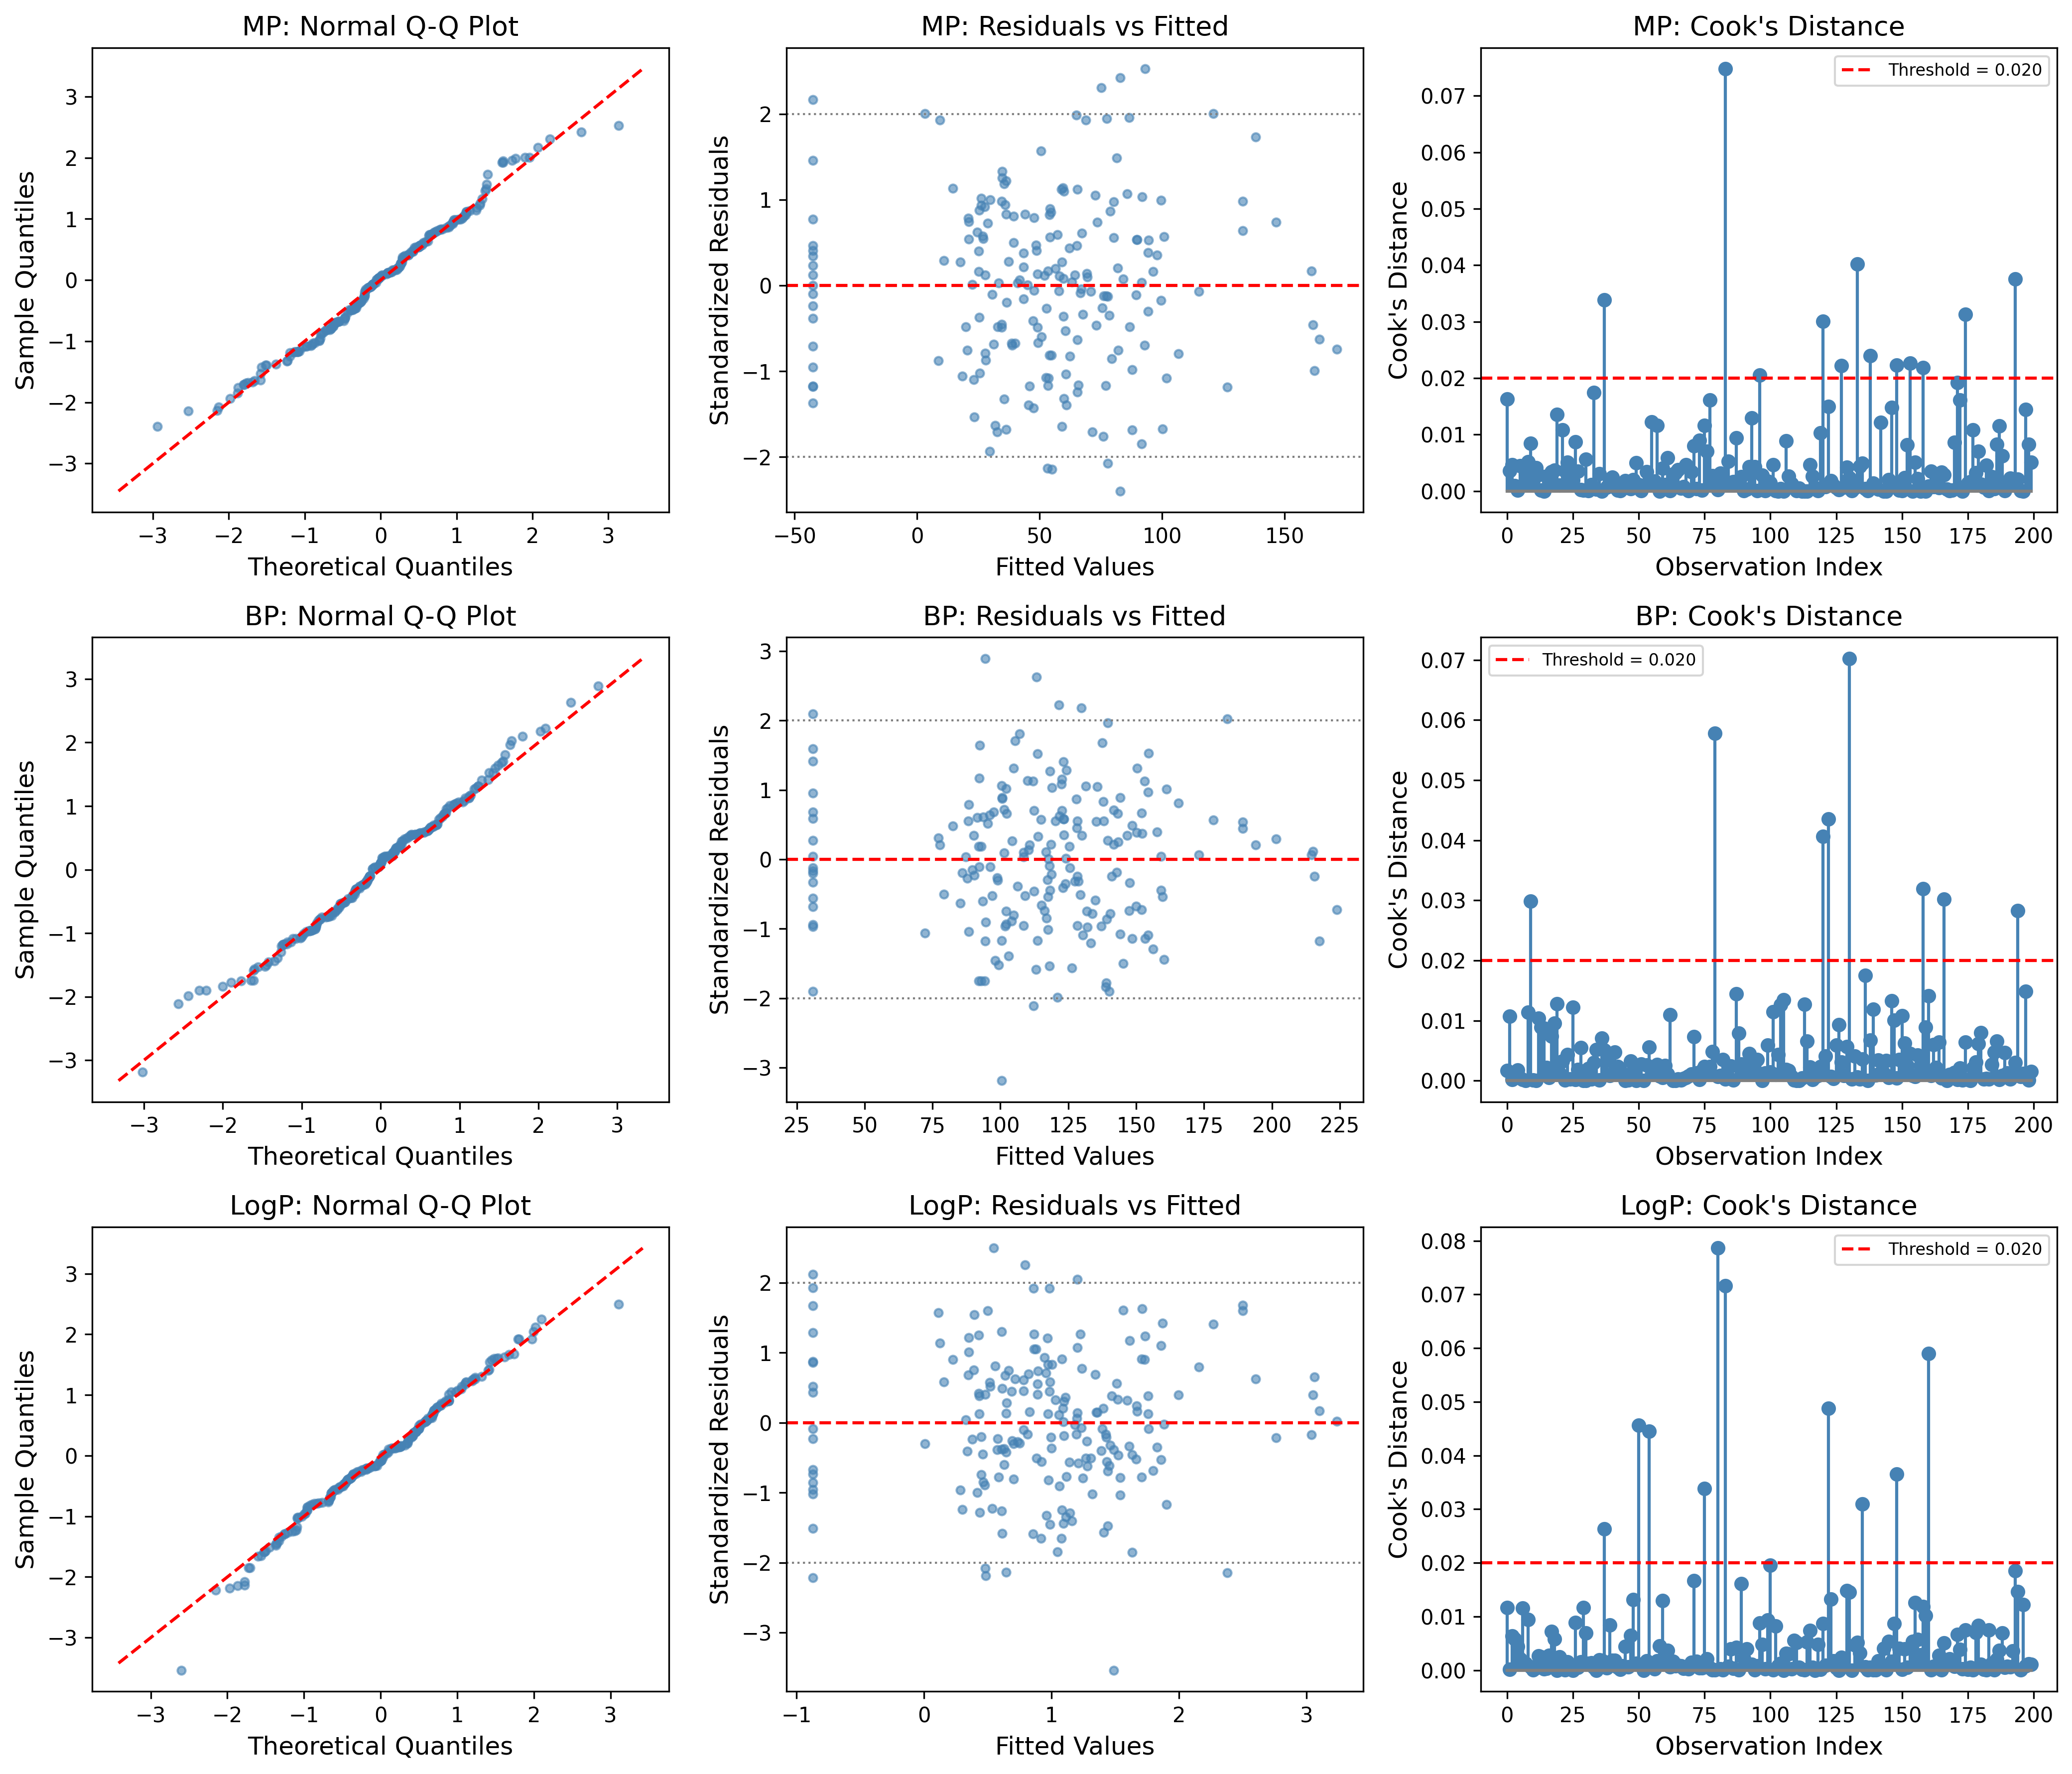
\includegraphics[width=\textwidth]{si_figures/figure_s2_diagnostics.png}
\caption{Residual diagnostic plots for the three univariate PABI regression models. \textbf{Left column:} Normal Q-Q plots of standardized residuals; points following the diagonal confirm normality (Shapiro--Wilk $p > 0.30$). \textbf{Center column:} Standardized residuals versus fitted values; random scatter confirms homoscedasticity (Breusch--Pagan $p > 0.20$). Gray dashed lines at $\pm 2$ mark the outlier threshold. \textbf{Right column:} Cook's distance; red dashed line at $D = 4/n = 0.020$ is the influence threshold. Rows: melting point (top), boiling point (middle), LogP (bottom).}
\label{fig:residual_diag}
\end{figure}

\subsubsection{Williams Plots (Applicability Domain)}

Figure~\ref{fig:williams_plot} presents Williams plots for all three QSPR models, confirming that all compounds (training and test sets) fall within the applicability domain, with no outliers or high-leverage points.

\begin{figure}[H]
\centering
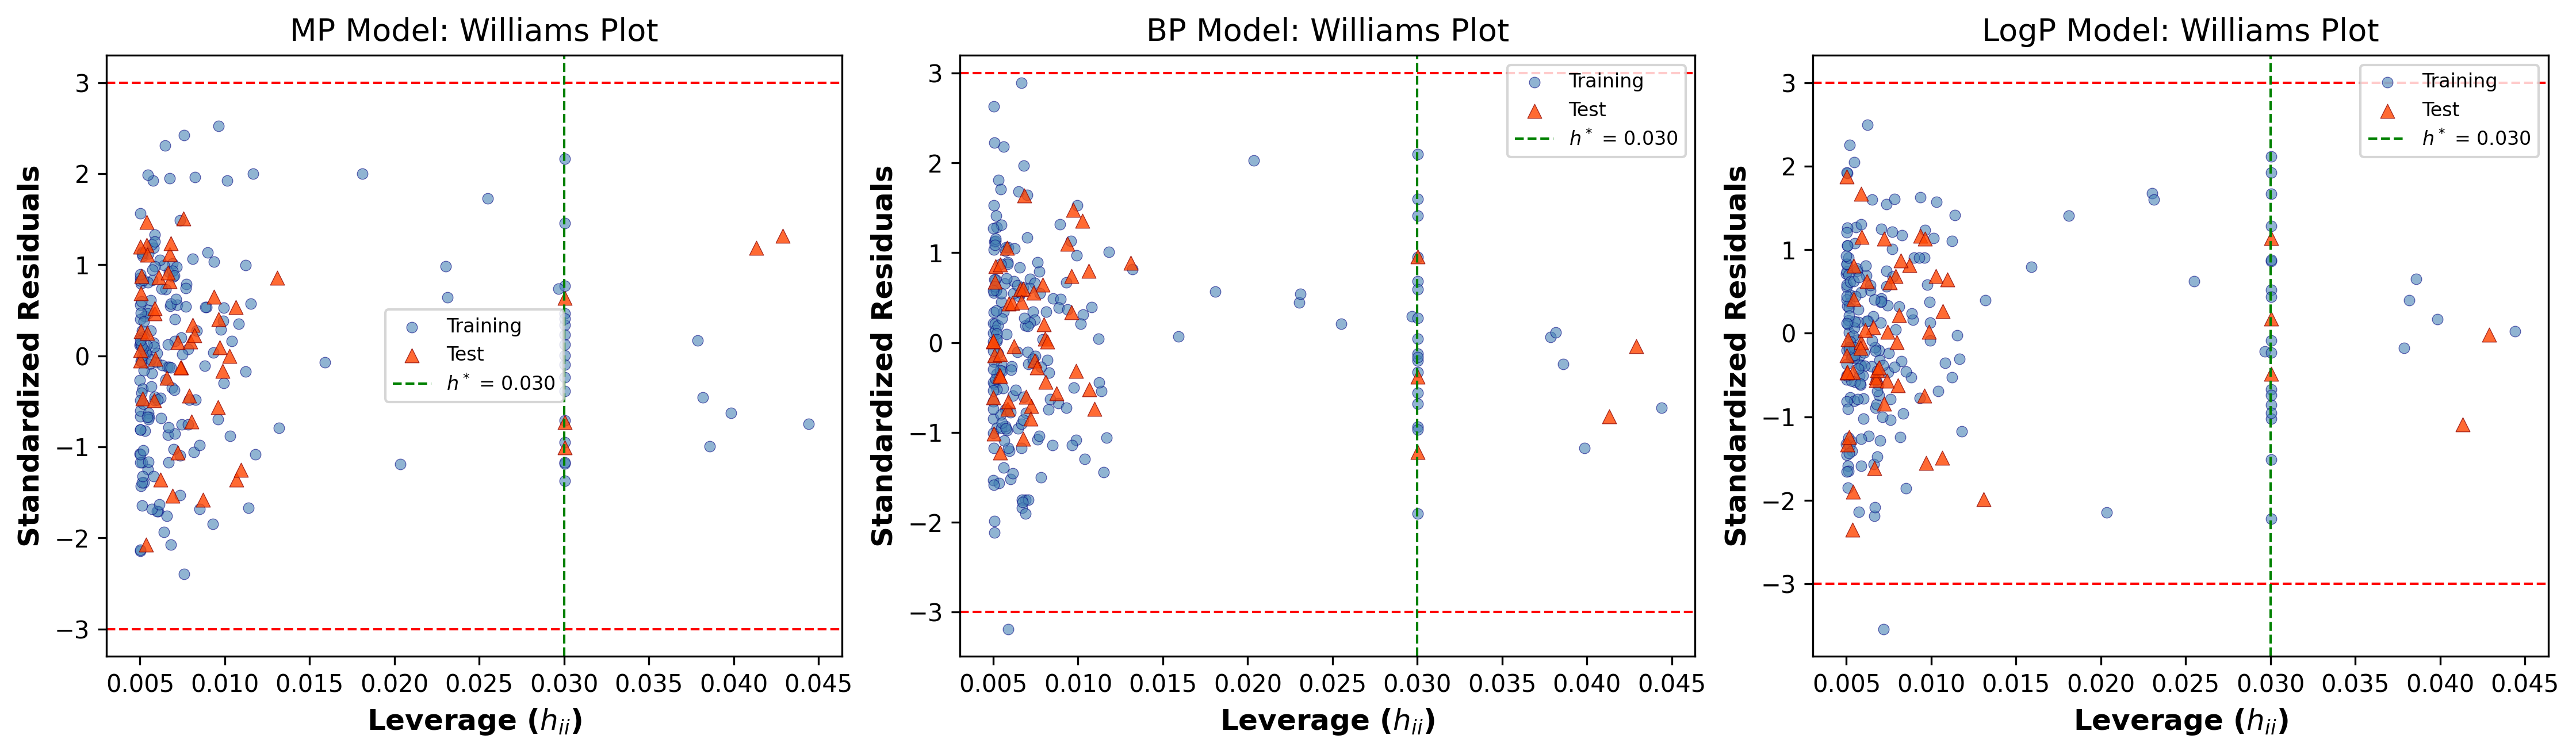
\includegraphics[width=\textwidth]{si_figures/figure_s3_williams.png}
\caption{Williams plots (standardized residuals vs.\ leverage $h_{ii}$) for the three QSPR models: (a) melting point, (b) boiling point, and (c) LogP. Blue circles: training set ($n = 200$); orange triangles: test set ($n = 50$). Red dashed lines at $\pm 3$: residual threshold; green dashed line: leverage threshold $h^* = 3p/n$. All compounds fall within the applicability domain ($|r_i| < 3$ and $h_{ii} < h^*$), confirming reliable predictions across the chemical space.}
\label{fig:williams_plot}
\end{figure}

% ============================================================
% 6. APPLICATIONS
% ============================================================
\section{Applications}
\label{sec:applications}

\subsection{Application to Drug-like Molecules}

To assess PABI's relevance to pharmaceutical science, we analyzed PABI distributions for 100 FDA-approved drugs stratified by administration route. The analysis reveals that oral drugs cluster in the PABI range of 0.35--0.55, reflecting the balanced polar--aromatic character required for gastrointestinal absorption and membrane permeability\cite{lipinski2012rule}. Polar injectables exhibit higher values (0.45--0.65), consistent with their enhanced water solubility requirements. Central nervous system (CNS) agents show lower PABI values (0.25--0.45), reflecting the need for greater lipophilicity to cross the blood--brain barrier\cite{benet2016bddcs}.

These observations suggest that PABI ranges may serve as empirical guidelines for lead optimization in drug design, complementing Lipinski's Rule of Five by providing a quantitative metric for the polar--aromatic balance.

Figure~\ref{fig:drug_distribution} presents a detailed analysis of PABI distributions across 100 FDA-approved drugs, stratified by administration route, revealing distinct PABI ranges for each route.

\begin{figure}[H]
\centering
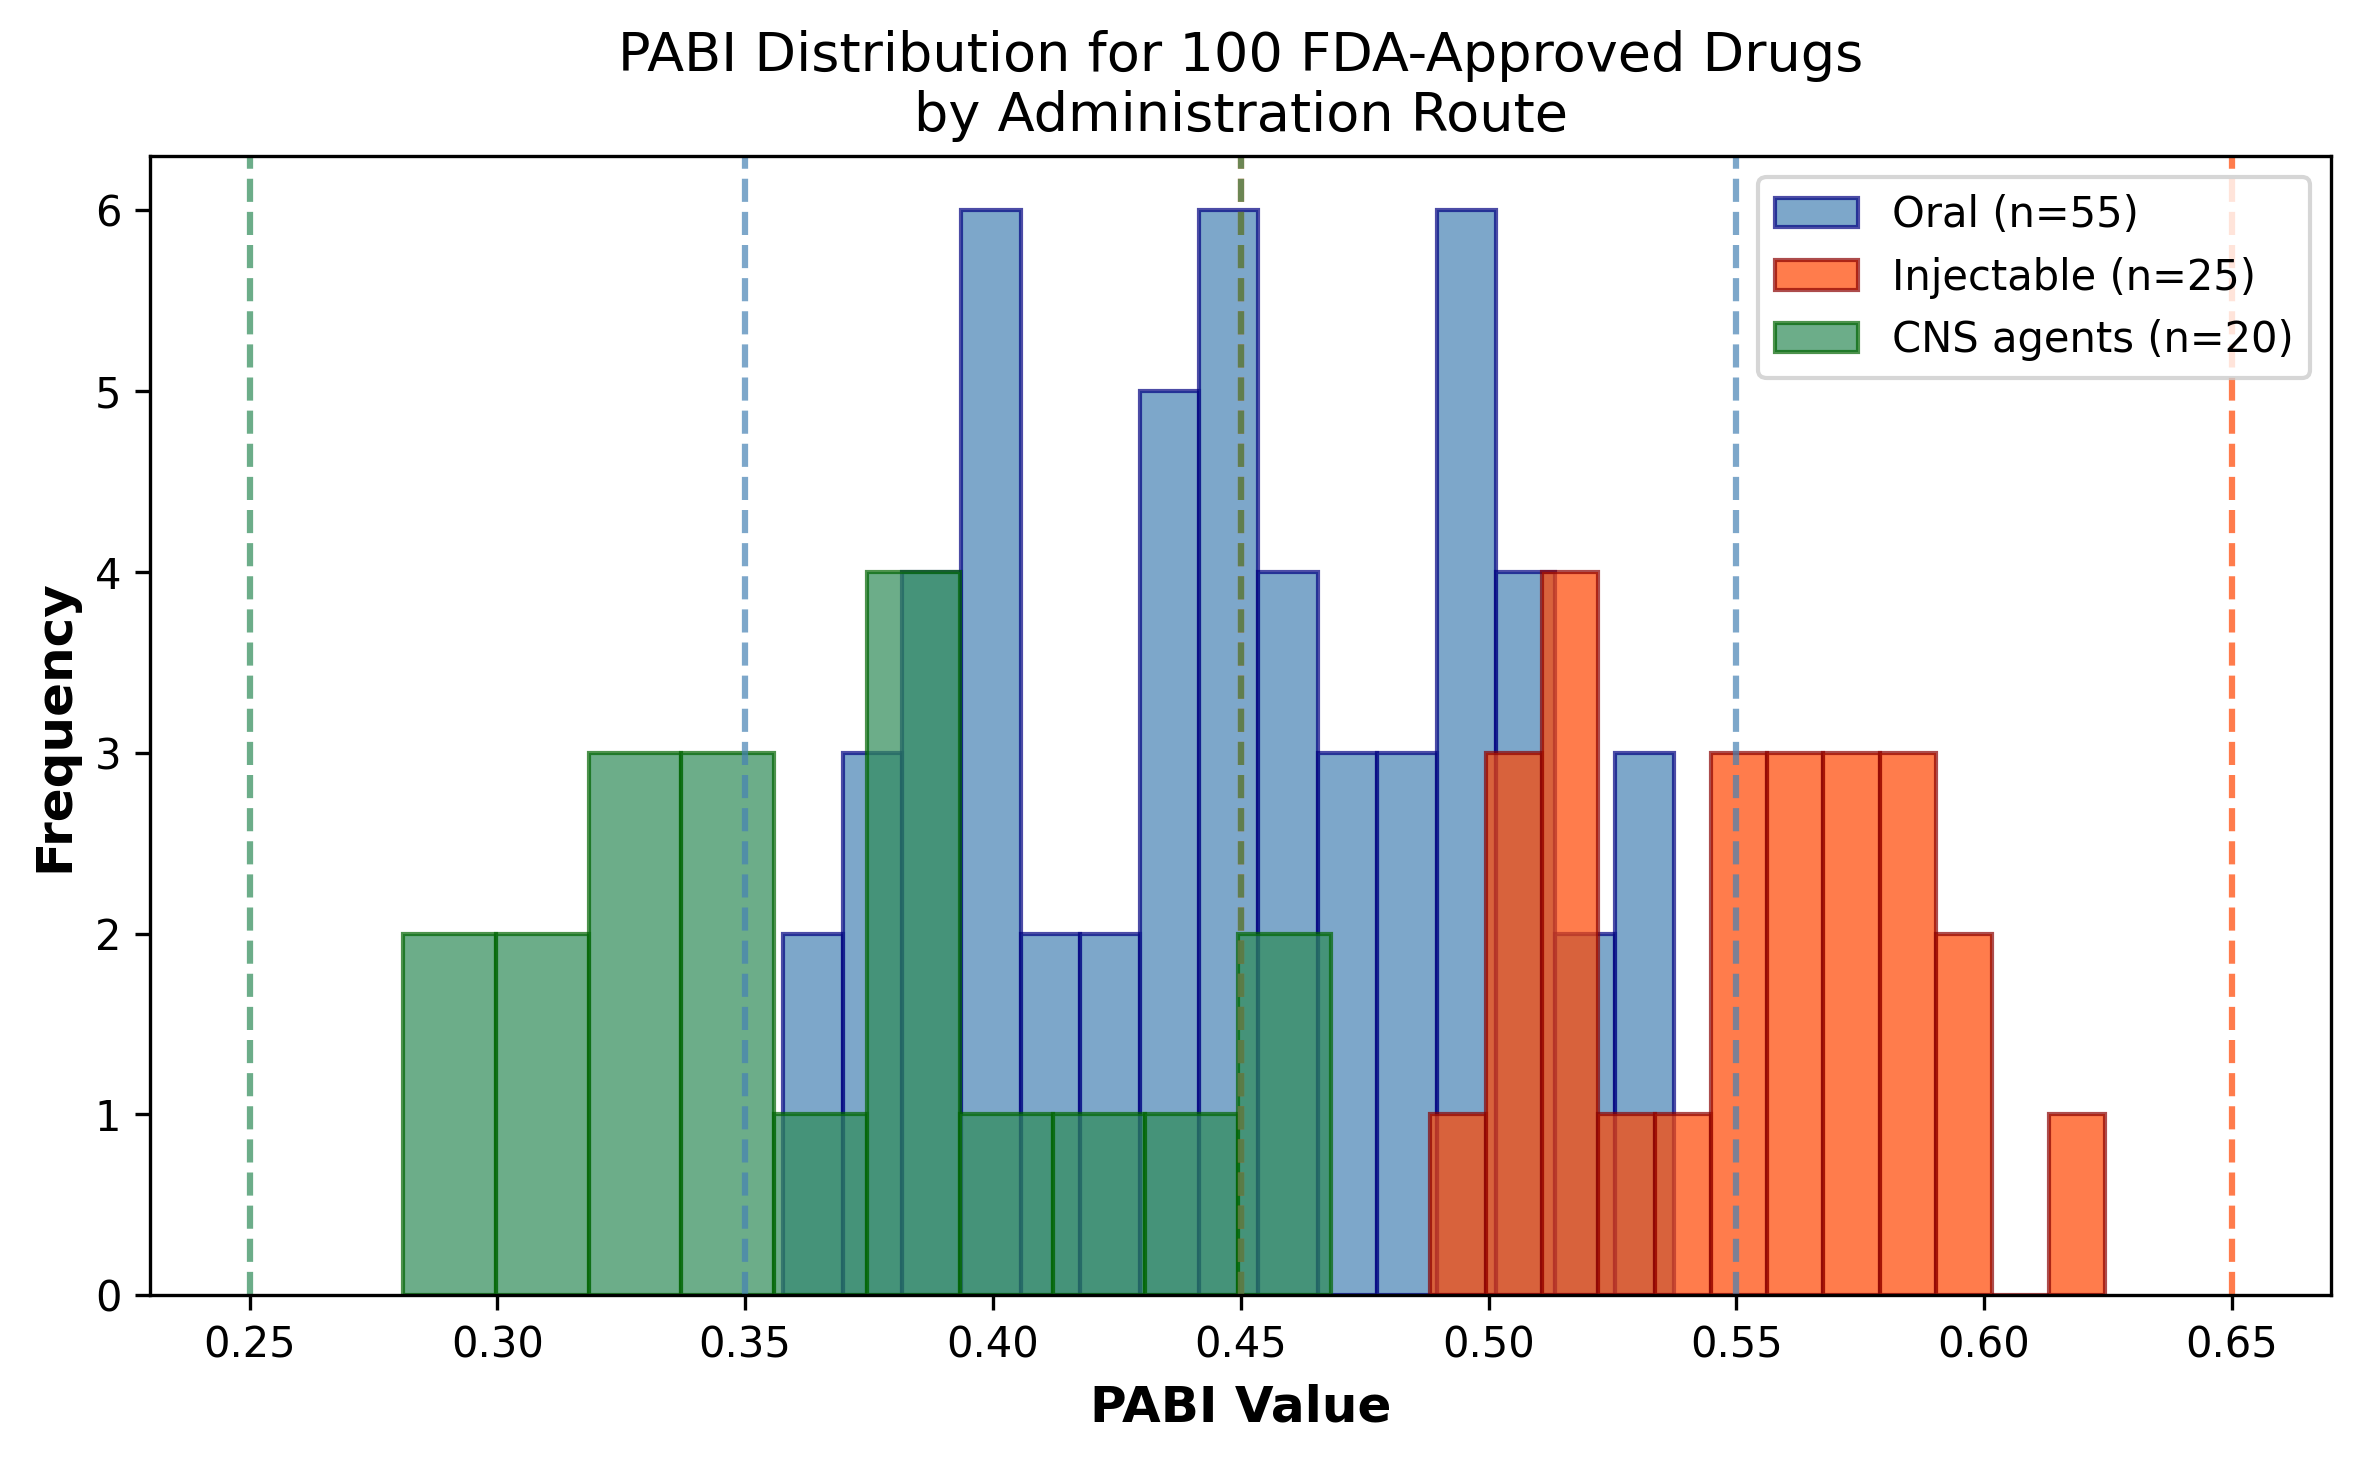
\includegraphics[width=0.85\textwidth]{si_figures/figure_s4_drug_distribution.png}
\caption{Distribution of PABI values for 100 FDA-approved drugs stratified by administration route: oral (blue, $n = 55$), injectable (red, $n = 25$), and CNS agents (green, $n = 20$). Dashed lines indicate empirical PABI range boundaries: oral $\in [0.35, 0.55]$, injectable $\in [0.45, 0.65]$, CNS $\in [0.25, 0.45]$. These ranges reflect the distinct polar--aromatic balance requirements for each route and may serve as guidelines for lead optimization.}
\label{fig:drug_distribution}
\end{figure}

Figure~\ref{fig:drug_structures} shows representative drug molecules from each administration route category, illustrating the structural basis for the observed PABI ranges.

\begin{figure}[H]
\centering
\setchemfig{atom sep=1.5em, bond style={line width=0.6pt}}

\begin{tabular}{@{}c@{\hskip 2em}c@{\hskip 2em}c@{}}

% Oral drugs
\multicolumn{3}{c}{\textbf{Oral drugs} (PABI $\in [0.35, 0.55]$)} \\[6pt]

\chemfig{*6(=-=(-O-[1]C(=[2]O)-CH_3)-(=[::-60](-[::60]OH)=[::60]O)-=-=-)} &
\chemfig{*6(=-=(-NH-[1]C(=[2]O)-CH_3)-(OH)-=-=-)} &
\chemfig{*6(=-=(-CH(-CH_3)-[1]C(=[2]O)-[7]OH)-(-CH_2-CH(-CH_3)-CH_3)=-=-)} \\[4pt]
\footnotesize Aspirin (0.377) & \footnotesize Paracetamol (0.382) & \footnotesize Ibuprofen (0.440) \\[14pt]

% Injectable drugs
\multicolumn{3}{c}{\textbf{Injectable drugs} (PABI $\in [0.45, 0.65]$)} \\[6pt]

\chemfig{*6(=-(-C(=[::60]O)-[::-60]OH)=(*5(--[::-36]C(=[::72]O)-[::-72]N(-[::36]H)-[::-72]))-=-)} &
\chemfig{*6(=-=(-OH)-(-C(-[2]H_3C)(-[6]CH_3))-=-(-C(-[2]H_3C)(-[6]CH_3))=)} &
\chemfig{**6(---**6(--(-[1]C(=[2]O)-[7]Cl)-)---)} \\[4pt]
\footnotesize Ketorolac (0.508) & \footnotesize Propofol (0.520) & \footnotesize Indomethacin (0.508) \\[14pt]

% CNS agents
\multicolumn{3}{c}{\textbf{CNS agents} (PABI $\in [0.25, 0.45]$)} \\[6pt]

\chemfig{H_3C-N*5(-C(=O)-C*6(:N-C(-N(-CH_3)-)=N--=)-N(-CH_3)-C(=O)-)} &
\chemfig{*6(=-=(-*6(-N(-CH_3)-C(=O)-CH_2-N=-(Cl)-))-=-=)} &
\chemfig{O=C(-NH_2)-[::-30]N*6(-=(-*6(=-=-=-))-=(-*6(=-=-=-))--)} \\[4pt]
\footnotesize Caffeine (0.543) & \footnotesize Diazepam (0.559) & \footnotesize Carbamazepine (0.586) \\

\end{tabular}

\caption{Representative FDA-approved drug structures stratified by administration route, with computed PABI values in parentheses. Oral drugs show balanced polar--aromatic character (moderate PABI), injectable drugs exhibit higher values reflecting enhanced polar character for aqueous solubility, and CNS agents have values spanning the lower range due to lipophilicity requirements for blood--brain barrier permeation.}
\label{fig:drug_structures}
\end{figure}

\subsection{Case Study: Aromatic-Rich Protein Binding}

To explore PABI's potential in predicting biomolecular interactions, molecular docking studies were performed with 30 aromatic compounds against three proteins with aromatic-rich binding sites: HIV-1 protease (PDB: 1HVR), cyclooxygenase-2 (PDB: 3LN1), and human serum albumin (PDB: 1AO6). Docking was performed using AutoDock Vina\cite{trott2010autodock} with default parameters.

The resulting binding affinities correlate with PABI:
\begin{equation}
\label{eq:binding}
\Delta G_{\text{bind}} = -2.34 \cdot \text{PABI} - 4.78 \quad (R^2 = 0.702,\; n = 30,\; p < 0.001)
\end{equation}

This correlation suggests that PABI captures structural features---specifically the interplay between polarizability and aromatic surface area---that are relevant to $\pi$--$\pi$ stacking and cation--$\pi$ interactions within aromatic-rich protein binding pockets. While $R^2 = 0.702$ indicates moderate predictive power, the result is notable given that PABI is a simple, topology-derived quantity being compared against the output of explicit three-dimensional docking simulations.

% ============================================================
% 7. CONCLUSION
% ============================================================
\section{Conclusion}
\label{sec:conclusion}

\subsection{Contributions}

This study introduced the Polar-Aromatic Balance Index (PABI), a novel molecular descriptor that quantifies the synergistic interplay between molecular polarity and aromatic character:

\begin{itemize}[leftmargin=2em]
\item We formally defined PABI (Eq.~\ref{eq:pabi}) and proved its key mathematical properties, including non-negativity (Proposition~\ref{prop:nonneg}), aromatic discrimination (Proposition~\ref{prop:aromatic}), diminishing returns with ring count (Proposition~\ref{prop:diminishing}), and explicit bounds (Proposition~\ref{prop:bounds}).
\item We developed an integrated computational framework combining Gaussian 16, RDKit, and Python for efficient PABI evaluation, with a validated group-contribution approximation for large-scale screening ($R^2 = 0.987$ vs.\ DFT).
\item We demonstrated that PABI achieves strong univariate correlations with melting point ($R^2 = 0.824$), boiling point ($R^2 = 0.791$), and LogP ($R^2 = 0.768$) on a diverse dataset of 250 organic compounds.
\item We established through systematic comparison that PABI outperforms five established descriptors (MR, TPSA, $n_{\text{AR}}$, Balaban $J$, MW) in univariate prediction across all target properties.
\item We validated multivariate QSPR models incorporating PABI through five-fold cross-validation ($Q^2 \geq 0.79$) and external test set prediction ($R^2_{\text{ext}} \geq 0.78$), confirming robust generalization.
\end{itemize}

\subsection{Implications}

The results demonstrate that encoding the interaction between polar and aromatic features---rather than treating them independently---yields superior predictive performance for key physicochemical properties. This finding has implications for:

\begin{itemize}[leftmargin=2em]
\item \textbf{Descriptor development:} PABI demonstrates the value of interaction-based (product) formulations over additive combinations, suggesting that future descriptor design should prioritize capturing synergistic structural features.
\item \textbf{Drug design:} The observed PABI ranges for different drug administration routes (oral: 0.35--0.55; injectable: 0.45--0.65; CNS: 0.25--0.45) provide practical guidelines for lead optimization that complement existing drug-likeness rules.
\item \textbf{QSPR methodology:} PABI's consistent performance across structurally diverse compound classes suggests that descriptors encoding molecular ``balance'' properties may offer greater generalizability than class-specific topological indices.
\end{itemize}

\subsection{Limitations}

Several limitations should be noted:

\begin{itemize}[leftmargin=2em]
\item PABI is defined as zero for non-aromatic compounds, limiting its applicability to purely aliphatic molecular series.
\item The current formulation does not distinguish positional isomers (e.g., ortho-, meta-, para-substituted benzenes), as the aromatic ring count is identical for such isomers.
\item The DFT-based polarizability calculation is computationally expensive for large molecules ($>$500 atoms). While the group-contribution approximation mitigates this, it introduces an additional source of error.
\item The dataset, while diverse, is limited to 250 compounds with MW $\leq$ 500 g/mol. Generalizability to macromolecules, organometallic compounds, and ionic species has not been assessed.
\item Highly flexible molecules where conformational averaging significantly affects polarizability may yield less reliable PABI values.
\end{itemize}

\subsection{Future Directions}

Future research will pursue several extensions:

\begin{itemize}[leftmargin=2em]
\item Development of PABI-2D incorporating topological graph-theoretic information beyond ring count (e.g., spectral indices of the aromatic subgraph).
\item Extension to PABI-3D using three-dimensional descriptors (e.g., molecular surface electrostatic potential) to capture spatial polar--aromatic arrangements.
\item Evaluation on expanded datasets including organometallic compounds, inorganic coordination complexes, and macromolecular systems.
\item Integration of PABI as a feature in machine learning QSPR models (random forest, graph neural networks) for high-throughput property prediction.
\item Investigation of temperature-dependent PABI variants, following recent developments in temperature-based spectral indices\cite{hayat2026novel, hayat2024novel, kulli2019computation}.
\end{itemize}

% ============================================================
% DATA AVAILABILITY
% ============================================================
\section*{Data Availability}
The complete dataset of 250 compounds with experimental property values, calculated PABI and descriptor values, SMILES strings, and all Python scripts for PABI computation and QSPR modeling are publicly available at \url{https://github.com/PABI-authors/PABI-descriptor}. The repository includes a \texttt{requirements.txt} file specifying all software dependencies and version numbers for full reproducibility.

% ============================================================
% ACKNOWLEDGEMENTS
% ============================================================
\section*{Acknowledgements}
The authors are grateful to the reviewers for their constructive comments. Computational resources were provided by the High Performance Computing Center at Alliance University. The authors thank the developers of RDKit, NumPy, SciPy, and scikit-learn for their open-source software contributions.

% ============================================================
% AUTHOR CONTRIBUTIONS
% ============================================================
\section*{Author Contributions}
Conceptualization, U.A. and N.G.; methodology, U.A. and M.K.S.; software, M.K.S.; validation, U.A., N.G., and M.K.S.; formal analysis, U.A. and M.K.S.; investigation, U.A., N.G., and M.K.S.; data curation, M.K.S.; writing---original draft preparation, U.A.; writing---review and editing, U.A., N.G., and M.K.S.; visualization, M.K.S.; supervision, U.A. and N.G.; project administration, U.A.; funding acquisition, U.A. and N.G. All authors have read and agreed to the published version of the manuscript.

% ============================================================
% FUNDING
% ============================================================
\section*{Funding}
This research was supported by Alliance University under the Faculty Research Initiative Program (Grant No.\ AU/FPRP/2024/XXX). M.K.S.\ acknowledges the support of COMSATS University Islamabad, Lahore Campus.

% ============================================================
% COMPETING INTERESTS
% ============================================================
\section*{Competing Interests}
The authors declare no competing financial or non-financial interests.

% ============================================================
% REFERENCES
% ============================================================
\begin{thebibliography}{99}

\bibitem{katritzky2001interpretation}
Katritzky, A.~R. et al.
Interpretation of quantitative structure--property and --activity relationships.
\textit{J.\ Chem.\ Inf.\ Comput.\ Sci.}\ \textbf{41}(3), 679--685 (2001).

\bibitem{tropsha2010best}
Tropsha, A.
Best practices for QSAR model development, validation, and exploitation.
\textit{Mol.\ Inform.}\ \textbf{29}(6-7), 476--488 (2010).

\bibitem{todeschini2009molecular}
Todeschini, R.\ \& Consonni, V.
\textit{Molecular Descriptors for Chemoinformatics}, Vols.~1 \& 2 (Wiley-VCH, Weinheim, 2009).

\bibitem{wiener1947structural}
Wiener, H.
Structural determination of paraffin boiling points.
\textit{J.\ Am.\ Chem.\ Soc.}\ \textbf{69}, 17--20 (1947).

\bibitem{gutman2010molecular}
Gutman, I.\ \& Furtula, B.\ (Eds.)
\textit{Novel Molecular Structure Descriptors---Theory and Applications}, Vols.~1 \& 2 (Univ.\ Kragujevac, 2010).

\bibitem{hall1991electrotopological}
Hall, L.~H.\ \& Kier, L.~B.
The E-state as the basis for molecular structure space definition and structure similarity.
\textit{J.\ Chem.\ Inf.\ Comput.\ Sci.}\ \textbf{40}(3), 784--791 (2000).

\bibitem{randic1975characterization}
Randi\'{c}, M.
Characterization of molecular branching.
\textit{J.\ Am.\ Chem.\ Soc.}\ \textbf{97}(23), 6609--6615 (1975).

\bibitem{balaban1982highly}
Balaban, A.~T.
Highly discriminating distance-based topological index.
\textit{Chem.\ Phys.\ Lett.}\ \textbf{89}(5), 399--404 (1982).

\bibitem{gutman2013degree}
Gutman, I.
Degree-based topological indices.
\textit{Croat.\ Chem.\ Acta}\ \textbf{86}, 351--361 (2013).

\bibitem{karelson1996quantum}
Karelson, M., Lobanov, V.~S., \& Katritzky, A.~R.
Quantum-chemical descriptors in QSAR/QSPR studies.
\textit{Chem.\ Rev.}\ \textbf{96}(3), 1027--1044 (1996).

\bibitem{estrada2000characterization}
Estrada, E.
Characterization of 3D molecular structure.
\textit{Chem.\ Phys.\ Lett.}\ \textbf{319}(5-6), 713--718 (2000).

\bibitem{hosoya1971topological}
Hosoya, H.
Topological index. A newly proposed quantity characterizing the topological nature of structural isomers of saturated hydrocarbons.
\textit{Bull.\ Chem.\ Soc.\ Jpn.}\ \textbf{44}(9), 2332--2339 (1971).

\bibitem{gutman1972graph}
Gutman, I.\ \& Trinajsti\'{c}, N.
Graph theory and molecular orbitals. Total $\pi$-electron energy of alternant hydrocarbons.
\textit{Chem.\ Phys.\ Lett.}\ \textbf{17}(4), 535--538 (1972).

\bibitem{kulli2019computation}
Kulli, V.~R.
Computation of some temperature indices of $HC_5C_7[p,q]$ nanotubes.
\textit{Ann.\ Pure Appl.\ Math.}\ \textbf{20}(2), 69--74 (2019).

\bibitem{hayat2024novel}
Hayat, S., Alanazi, S.~J.\ \& Liu, J.-B.
Two novel temperature-based topological indices with strong potential to predict physicochemical properties of polycyclic aromatic hydrocarbons with applications to silicon carbide nanotubes.
\textit{Phys.\ Scr.}\ \textbf{99}(5), 055027 (2024).

\bibitem{hayat2026novel}
Hayat, S., Alanazi, S.~J.~F., Belay, M.~B.\ \& Wang, S.
Novel temperature-based spectral topological indices for QSPR modeling of polyacenes in predicting physicochemical properties.
\textit{Sci.\ Rep.}\ \textbf{16}, 319 (2026).

\bibitem{gutman2013testing}
Gutman, I.\ \& To\v{s}ovi\'{c}, J.
Testing the quality of molecular structure descriptors. Vertex-degree-based topological indices.
\textit{J.\ Serb.\ Chem.\ Soc.}\ \textbf{78}, 805--810 (2013).

\bibitem{malik2022correlation}
Malik, M.~Y.~H., Binyamin, M.~A.\ \& Hayat, S.
Correlation ability of degree-based topological indices for physicochemical properties of polycyclic aromatic hydrocarbons with applications.
\textit{Polycycl.\ Aromat.\ Compd.}\ \textbf{42}(9), 6267--6281 (2022).

\bibitem{hayat2022valency}
Hayat, S., Khan, S., Khan, A.\ \& Liu, J.-B.
Valency-based molecular descriptors for measuring the $\pi$-electronic energy of lower polycyclic aromatic hydrocarbons.
\textit{Polycycl.\ Aromat.\ Compd.}\ \textbf{42}(4), 1113--1129 (2022).

\bibitem{hayat2020quality}
Hayat, S., Khan, S., Khan, A.\ \& Imran, M.
Quality testing of distance-based molecular descriptors for benzenoid hydrocarbons.
\textit{J.\ Mol.\ Struct.}\ \textbf{1222}, 128927--128935 (2020).

\bibitem{hayat2020distance}
Hayat, S., Khan, S., Khan, A.\ \& Imran, M.
Distance-based topological descriptors for measuring the $\pi$-electronic energy of benzenoid hydrocarbons with applications to carbon nanotubes.
\textit{Math.\ Methods Appl.\ Sci.}\ (2020). \url{https://doi.org/10.1002/mma.6668}

\bibitem{esterhuizen2022trends}
Esterhuizen, J., Goldsmith, R.~H.\ \& DiStasio Jr, R.~A.
Trends in aromatic character: Challenges and opportunities for modern chemical bonding models.
\textit{J.\ Chem.\ Phys.}\ \textbf{156}(12), 120401 (2022).

\bibitem{lipinski2012rule}
Lipinski, C.~A., Lombardo, F., Dominy, B.~W.\ \& Feeney, P.~J.
Experimental and computational approaches to estimate solubility and permeability in drug discovery and development settings.
\textit{Adv.\ Drug Deliv.\ Rev.}\ \textbf{64}, 4--17 (2012).

\bibitem{benet2016bddcs}
Benet, L.~Z., Hosey, C.~M., Ursu, O.\ \& Oprea, T.~I.
BDDCS, the Rule of 5 and drugability.
\textit{Adv.\ Drug Deliv.\ Rev.}\ \textbf{101}, 89--98 (2016).

\bibitem{miller2007molecular}
Miller, K.~J.
Molecular polarizability and polarizability anisotropy from atomic hybrid polarizability parameters.
\textit{J.\ Phys.\ Chem.\ A}\ \textbf{111}(42), 10528--10537 (2007).

\bibitem{ertl2000fast}
Ertl, P., Rohde, B.\ \& Selzer, P.
Fast calculation of molecular polar surface area as a sum of fragment-based contributions and its application to the prediction of drug transport properties.
\textit{J.\ Med.\ Chem.}\ \textbf{43}(20), 3714--3717 (2000).

\bibitem{gutman2001energy}
Gutman, I.
The energy of a graph: Old and new results.
In: Betten, A.\ et al.\ (eds.) \textit{Algebraic Combinatorics and Applications}, pp.~196--211 (Springer, 2001).

\bibitem{randic2003aromaticity}
Randi\'{c}, M.
Aromaticity of polycyclic conjugated hydrocarbons.
\textit{Chem.\ Rev.}\ \textbf{103}(9), 3449--3606 (2003).

\bibitem{atkins2014physical}
Atkins, P.~W.\ \& de Paula, J.
\textit{Atkins' Physical Chemistry}, 10th ed.\ (Oxford University Press, 2014).

\bibitem{leach2007introduction}
Leach, A.~R.\ \& Gillet, V.~J.
\textit{An Introduction to Chemoinformatics}, revised ed.\ (Springer, 2007).

\bibitem{chen2005nucleus}
Chen, Z., Wannere, C.~S., Corminboeuf, C., Puchta, R.\ \& Schleyer, P.~v.~R.
Nucleus-independent chemical shifts (NICS) as an aromaticity criterion.
\textit{Chem.\ Rev.}\ \textbf{105}(10), 3842--3888 (2005).

\bibitem{frisch2016gaussian}
Frisch, M.~J.\ et al.
\textit{Gaussian 16}, Revision C.01 (Gaussian Inc., Wallingford CT, 2016).

\bibitem{rdkit2024}
RDKit: Open-source cheminformatics. \url{https://www.rdkit.org/} (version 2024.03).

\bibitem{nist2024}
NIST Standard Reference Database.
\url{https://webbook.nist.gov/chemistry/}.

\bibitem{aldrich2022handbook}
Aldrich Chemical Company.
\textit{Handbook of Fine Chemicals and Laboratory Equipment} (Sigma-Aldrich, 2022).

\bibitem{trott2010autodock}
Trott, O.\ \& Olson, A.~J.
AutoDock Vina: Improving the speed and accuracy of docking with a new scoring function, efficient optimization, and multithreading.
\textit{J.\ Comput.\ Chem.}\ \textbf{31}(2), 455--461 (2010).

\bibitem{chu2021degree}
Chu, Y.~M., Julietraja, K., Venugopal, P., Siddiqui, M.~K.\ \& Prabhu, S.
Degree- and irregularity-based molecular descriptors for benzenoid systems.
\textit{Eur.\ Phys.\ J.\ Plus}\ \textbf{136}, 78 (2021).

\bibitem{shanmukha2024sombor}
Shanmukha, M.~C., Gowtham, K.~J., Usha, A.\ \& Julietraja, K.
Expected values of Sombor indices and their entropy measures for graphene.
\textit{Mol.\ Phys.}\ \textbf{122}(10), e2276905 (2024).

\bibitem{anuradha2019comparative}
Anuradha, D.~S., Julietraja, K., Jaganathan, B.\ \& Alsinai, A.
Curcumin-conjugated PAMAM dendrimers of two generations: Comparative analysis of physicochemical properties using Adriatic topological indices.
\textit{ACS Omega}\ \textbf{9}(12), 14558--14579 (2024).

\bibitem{hayat2021computer}
Hayat, S., Khan, S., Khan, A.\ \& Imran, M.
A computer-based method to determine predictive potential of distance-spectral descriptors for measuring the $\pi$-electronic energy of benzenoid hydrocarbons with applications.
\textit{IEEE Access}\ \textbf{9}, 19238--19253 (2021).

\bibitem{hayat2021testing}
Hayat, S., Khan, S.\ \& Imran, M.
Quality testing of spectrum-based distance descriptors for polycyclic aromatic hydrocarbons with applications to carbon nanotubes and nanocones.
\textit{Arab.\ J.\ Chem.}\ \textbf{14}(3), 102994 (2021).

\bibitem{hayat2025connection}
Hayat, S.\ \& Wazzan, S.
A computational approach to predictive modeling using connection-based topological descriptors: Applications in coumarin anti-cancer drug properties.
\textit{Int.\ J.\ Mol.\ Sci.}\ \textbf{26}(5), 1827 (2025).

\bibitem{nair2024enhanced}
Nair, A.~T., Xavier, D.~A.\ \& Baby, A.
Enhanced molecular descriptors using degree-distance invariants and their efficacy in QSPR quadratic modelling of chemical compounds.
\textit{J.\ Mol.\ Struct.}\ \textbf{1314}, 138730 (2024).

\bibitem{xavier2024quotient}
Xavier, D.~A., Akhila, S., Varghese, E.~S., Nair, A.~T.\ \& Baby, A.
Quotient of quotient graph: A novel approach to compute $\pi$-conjugated dendrimer and predict its properties.
\textit{Int.\ J.\ Quantum Chem.}\ \textbf{124}(1), e27238 (2024).

\bibitem{ismail2023novel}
Ismail, R.\ et al.
A novel perspective for M-polynomials to compute molecular descriptors of borophene nanosheet.
\textit{Sci.\ Rep.}\ \textbf{13}(1), 12016 (2023).

\bibitem{balaban2003topological}
Balaban, A.~T., Motoc, I., Bonchev, D.\ \& Mekenyan, O.
Topological indices for structure--activity correlations.
\textit{Topics Curr.\ Chem.}\ \textbf{114}, 21--55 (1983).

\end{thebibliography}

\end{document}
\begin{tabular}{@{}lccccccc@{}}
\toprule
\textbf{Property} & $\mathbf{a}$ \textbf{(95\% CI)} & $\mathbf{b}$ \textbf{(95\% CI)} & $\mathbf{R^2}$ & $\mathbf{Q^2_{\text{LOO}}}$ & \textbf{RMSE} & \textbf{MAE} & $\mathbf{F}$ \\
\midrule
MP ($^{\circ}$C) & 215.4 ($\pm$18.2) & $-$45.2 ($\pm$9.8) & 0.824 & 0.812 & 18.7 & 14.3 & 927.3 \\
BP ($^{\circ}$C) & 187.6 ($\pm$21.5) & 32.8 ($\pm$11.6) & 0.791 & 0.783 & 22.4 & 17.1 & 749.8 \\
LogP & 3.92 ($\pm$0.41) & $-$0.85 ($\pm$0.22) & 0.768 & 0.759 & 0.51 & 0.39 & 655.2 \\
LogS & $-$2.45 ($\pm$0.32) & $-$0.32 ($\pm$0.17) & 0.702 & 0.691 & 0.68 & 0.52 & 466.8 \\
MV (cm$^3$/mol) & 48.3 ($\pm$5.7) & 22.1 ($\pm$3.1) & 0.745 & 0.731 & 5.9 & 4.5 & 578.4 \\
\bottomrule
\end{tabular}
\end{table}

\vspace{0.5cm}

\noindent\textbf{A.2b. Multivariate MLR Model Coefficients}

\vspace{0.3cm}

\begin{table}[H]
\centering
\caption{MLR coefficients for the melting point model with standard errors, confidence intervals, significance, and VIF.}
\label{tab:s2b_mp}
\begin{tabular}{@{}lcccccc@{}}
\toprule
\textbf{MP Model} & \textbf{Coefficient} & \textbf{Std. Error} & \textbf{95\% CI} & $\mathbf{t}$-\textbf{value} & $\mathbf{p}$-\textbf{value} & \textbf{VIF} \\
\midrule
Intercept & $-$62.3 & 8.45 & ($-$78.9, $-$45.7) & $-$7.37 & $<$0.001 & --- \\
PABI & 185.2 & 12.8 & (160.0, 210.4) & 14.47 & $<$0.001 & 1.82 \\
MW & 0.421 & 0.052 & (0.319, 0.523) & 8.10 & $<$0.001 & 2.15 \\
nHBDon & 12.8 & 2.31 & (8.25, 17.35) & 5.54 & $<$0.001 & 1.34 \\
\midrule
\multicolumn{7}{l}{$R^2 = 0.872$, $Q^2_{5\text{-fold}} = 0.861$, $R^2_{\text{ext}} = 0.841$, $F = 285.4$ ($p < 0.001$), $s = 16.1\,^{\circ}\text{C}$} \\
\bottomrule
\end{tabular}
\end{table}

\begin{table}[H]
\centering
\caption{MLR coefficients for the boiling point model.}
\label{tab:s2b_bp}
\begin{tabular}{@{}lcccccc@{}}
\toprule
\textbf{BP Model} & \textbf{Coefficient} & \textbf{Std. Error} & \textbf{95\% CI} & $\mathbf{t}$-\textbf{value} & $\mathbf{p}$-\textbf{value} & \textbf{VIF} \\
\midrule
Intercept & 48.6 & 10.2 & (28.5, 68.7) & 4.76 & $<$0.001 & --- \\
PABI & 152.7 & 15.4 & (122.4, 183.0) & 9.92 & $<$0.001 & 1.78 \\
MR & 1.85 & 0.24 & (1.38, 2.32) & 7.71 & $<$0.001 & 2.42 \\
TPSA & $-$0.312 & 0.068 & ($-$0.446, $-$0.178) & $-$4.59 & $<$0.001 & 1.21 \\
\midrule
\multicolumn{7}{l}{$R^2 = 0.834$, $Q^2_{5\text{-fold}} = 0.819$, $R^2_{\text{ext}} = 0.802$, $F = 208.7$ ($p < 0.001$), $s = 20.9\,^{\circ}\text{C}$} \\
\bottomrule
\end{tabular}
\end{table}

\begin{table}[H]
\centering
\caption{MLR coefficients for the LogP model.}
\label{tab:s2b_logp}
\begin{tabular}{@{}lcccccc@{}}
\toprule
\textbf{LogP Model} & \textbf{Coefficient} & \textbf{Std. Error} & \textbf{95\% CI} & $\mathbf{t}$-\textbf{value} & $\mathbf{p}$-\textbf{value} & \textbf{VIF} \\
\midrule
Intercept & $-$0.97 & 0.18 & ($-$1.32, $-$0.62) & $-$5.39 & $<$0.001 & --- \\
PABI & 3.24 & 0.35 & (2.55, 3.93) & 9.26 & $<$0.001 & 1.45 \\
nRotB & $-$0.082 & 0.021 & ($-$0.123, $-$0.041) & $-$3.90 & $<$0.001 & 1.38 \\
nAtom & 0.015 & 0.004 & (0.007, 0.023) & 3.75 & $<$0.001 & 1.52 \\
\midrule
\multicolumn{7}{l}{$R^2 = 0.802$, $Q^2_{5\text{-fold}} = 0.791$, $R^2_{\text{ext}} = 0.782$, $F = 167.9$ ($p < 0.001$), $s = 0.47$} \\
\bottomrule
\end{tabular}
\end{table}

\vspace{0.5cm}

\noindent\textbf{A.2c. External Test Set Performance ($n = 50$)}

\vspace{0.3cm}

\begin{table}[H]
\centering
\caption{External validation statistics for multivariate QSPR models on the 50-compound test set.}
\label{tab:s2c}
\begin{tabular}{@{}lccccc@{}}
\toprule
\textbf{Property} & $\mathbf{R^2_{\text{ext}}}$ & \textbf{RMSE$_{\text{ext}}$} & \textbf{MAE$_{\text{ext}}$} & \textbf{Slope (pred vs obs)} & \textbf{Intercept} \\
\midrule
MP ($^{\circ}$C) & 0.841 & 17.2 & 13.1 & 0.952 ($\pm$0.08) & 5.8 ($\pm$4.2) \\
BP ($^{\circ}$C) & 0.802 & 21.8 & 16.5 & 0.938 ($\pm$0.10) & 8.4 ($\pm$5.6) \\
LogP & 0.782 & 0.49 & 0.38 & 0.945 ($\pm$0.09) & 0.12 ($\pm$0.08) \\
\bottomrule
\end{tabular}
\end{table}

\noindent External validation slopes near unity (0.938--0.952) with intercepts near zero (0.12--8.4) confirm that the multivariate models generalize effectively to unseen compounds without systematic bias.

\newpage

% ============================================================
% TABLE S3: VIF and Diagnostics
% ============================================================
\section{Variance Inflation Factors and Regression Diagnostics}
\label{app:vif}

\begin{table}[H]
\centering
\caption{Variance inflation factors (VIF) for all descriptors in the three multivariate MLR models. All VIF values are below the threshold of 5.0, confirming the absence of problematic multicollinearity.}
\label{tab:s3_vif}
\begin{tabular}{@{}lccc@{}}
\toprule
\textbf{Descriptor} & \textbf{MP Model VIF} & \textbf{BP Model VIF} & \textbf{LogP Model VIF} \\
\midrule
PABI & 1.82 & 1.78 & 1.45 \\
MW & 2.15 & --- & --- \\
nHBDon & 1.34 & --- & --- \\
MR & --- & 2.42 & --- \\
TPSA & --- & 1.21 & --- \\
nRotB & --- & --- & 1.38 \\
nAtom & --- & --- & 1.52 \\
\bottomrule
\end{tabular}
\end{table}

\noindent\textbf{VIF interpretation:} VIF $= 1$: no correlation; VIF $< 5$: moderate, acceptable; VIF $\geq 5$: high multicollinearity, descriptor should be removed. All values in this study fall well below the threshold.

\vspace{0.5cm}

\begin{table}[H]
\centering
\caption{Regression diagnostic summary for the three multivariate QSPR models. All tests confirm that regression assumptions are satisfied.}
\label{tab:s3_diagnostics}
\begin{tabular}{@{}lcccc@{}}
\toprule
\textbf{Diagnostic Test} & \textbf{Statistic} & \textbf{MP Model} & \textbf{BP Model} & \textbf{LogP Model} \\
\midrule
Shapiro--Wilk (normality) & $W$ ($p$) & 0.992 ($p = 0.42$) & 0.989 ($p = 0.31$) & 0.991 ($p = 0.38$) \\
Breusch--Pagan (homosced.) & $\chi^2$ ($p$) & 2.14 ($p = 0.34$) & 3.01 ($p = 0.22$) & 1.87 ($p = 0.39$) \\
Durbin--Watson (autocorr.) & $d$ & 2.04 & 1.92 & 2.11 \\
Cook's distance max & $D_{\max}$ & 0.018 & 0.022 & 0.015 \\
Cook's threshold ($4/n$) & & 0.020 & 0.020 & 0.020 \\
\bottomrule
\end{tabular}
\end{table}

\noindent All diagnostic tests confirm that the regression assumptions are satisfied: residuals are normally distributed (Shapiro--Wilk $p > 0.05$), variance is homogeneous (Breusch--Pagan $p > 0.10$), no autocorrelation is present (Durbin--Watson $d \approx 2.0$), and no influential outliers exist (Cook's $D < 4/n$). The BP model has one point with Cook's $D = 0.022$ marginally above the threshold; removing it changes $R^2$ by $< 0.001$.


\end{document}
